\documentclass[a4paper, 12pt]{book}

\usepackage[utf8]{inputenc}
\usepackage{blindtext}
\usepackage{graphicx}
\usepackage{pgfplotstable}
\usepackage{booktabs}
\usepackage{filecontents}
\usepackage{longtable}
\usepackage{float}
\usepackage[T1]{fontenc}
\usepackage{tocloft}
\usepackage[backend=biber]{biblatex}
\addbibresource{references.bib}
\usepackage[skip=5pt plus1pt, indent=0pt]{parskip}

\usepackage[hidelinks]{hyperref}
\hypersetup{
    linktoc=all
    allcolors=black
}

\graphicspath{
  {./images/}
  {./troubleshooting/}
  {./sourdough-starter/}
  {./troubleshooting/crumb-structures/}
  {./history/}
  {./images/external/}
  {./baking/}
  {./wheat-sourdough/}
}

\interfootnotelinepenalty=10000

\advance\cftsecnumwidth 0.5em\relax
\advance\cftsubsecindent 0.5em\relax
\advance\cftsubsecnumwidth 0.5em\relax
\begin{document}

\begin{titlepage}
	\centering
  \includegraphics[width=\textwidth]{cover-page}
  Version:
  \today
\end{titlepage}


\frontmatter

\tableofcontents

\chapter{Foreword}
Hopefully one day there is going to be an awesome foreword
by another break baker!

\chapter{Preface}
If there is the one food from Germany it is probably bread. There are thousands
of different varieties of bread in Germany. Making bread has been an integral part
of our culture. Beginning my studies in Göttingen for the first time I was faced
with buying bread on my own. In Germany that is no easy task
as the varieties of bread are endless. I started to check the packaging
of different bread types and noticed how there were surprisingly
many ingredients in most of the breads found in a common supermarket.


\chapter{Acknowledgements}
This book would not have been possible without the help of the community. Thank you very much for all the support. \\ \\


\begin{filecontents}{supporters.csv}
  \end{filecontents}

  {\large All supporters sorted by name}

  \pgfplotstableset{
  begin table=\begin{longtable},
  end table=\end{longtable},
  }

  \pgfplotstabletypeset[col sep=comma,
  header=true,
  columns={Name},      % display specified columns
  columns/Name/.style={column type=l,string type},
  % requires booktabs to place horiz rules
  every head row/.style={before row=\toprule, after row=\midrule\endhead},
  every last row/.style={after row=\bottomrule}
  ]{supporters.csv}


\mainmatter

\chapter{The history of sourdough}
Sourdough has been made since ancient times. The exact origins of fermented
bread are, however, unknown. One of the most ancient preserved
sourdough breads has been excavated in Switzerland.
However, based on recent research, some scientists speculate that sourdough
bread had already been made in 12000 BC in ancient Jordan \cite{jordan+bread}.

\includegraphics[width=\textwidth]{einkorn-crumb}

\chapter{How sourdough works}
In this chapter, we will cover the basics of how sourdough ferments.
First, we will look at the enzymatic reactions that take place
in your flour the moment you add water, triggering the fermentation
process. Then, in order to better understand this process, we will
learn more about the yeast and bacterial microorganisms involved.

\begin{figure}[!htb]
  \includegraphics[width=\textwidth]{infographic-enzymes}
  \caption{How amylases and proteases interact with flour}
  \label{infographic-enzymes}
\end{figure}

\section{Enzymatic reactions}

To understand the many enzymatic reactions that take place when flour
and water are mixed, we must first understand seeds and their role in
the lifecycle of wheat and other grains.

Seeds are the primary means by which many plants, including wheat,
reproduce. Each seed contains the embryo of another plant, and must
therefore contain all the nutrients that new plant requires to grow.

When the seed is dry, it is in hibernation mode and can sometimes be
stored for several years. The moment it comes into contact with water,
however, it begins to sprout. The seed turns into a germ, requiring the
stored nutrients to be converted into something the plant can use while
it grows. The catalyst that makes the associated reactions possible is water.

The seed typically contains the first prototypical leaves of the plant,
and can put down roots using the stored nutrients inside. Once those leaves
break through the soil and come into contact with the sunlight above, they
begin to photosynthesize. This process is the plant's engine, and with the
energy photosynthesis produces, the plant can continue to grow more roots,
enabling it to access additional nutrients from the soil. These additional
nutrients allow the plant to grow more leaves, increasing its photosynthetic
activity so that it can thrive in its new environment.

Of course, a ground flour can no longer sprout. But the enzymes that
trigger this process are still present. That's why it's important not to
mill grains at too high a temperature, as doing so could damage some of
these enzymes.

Normally, the grain seed shields the germ against pathogens. However, as the
grain is ground into flour, the contents of the seed are exposed. This is ideal
for our sourdough microorganisms.

Neither the yeast, considered a saprotrophic fungus, nor the bacteria can
prepare their own food. However, as the enzymes are activated, the food they
need becomes available, allowing them to feed and multiply.

The two main enzymes involved in this process are \textbf{amylase} and
\textbf{protease}. For reasons that will soon be clear, they are of the utmost
importance to the home baker, and their role in the making of sourdough is a
key puzzle piece to making better-tasting bread.

\subsection{Amylase}

Sometimes, when you chew on a potato or a piece of bread
for a long period of time, you'll begin to notice a sweet flavor in
your mouth. That's because your salivary glands produce amylase.
Amylase breaks down complex starch molecules into easily-digestible
sugars. The germ needs this to produce more plant matter, and your body
needs this to kick-start the digestive process. Normally, the microorganisms
on the surface of the grain can't consume the freed maltose molecules,
which remain hidden inside the germ. But as we grind the flour, a feeding
frenzy begins. Generally, the warmer the temperature, the faster this
reaction takes place. That's why a long fermentation is key to making
great bread. It takes time for the amylase to break down most of
the starch into simple sugars, which are not only consumed by the
yeast but are also essential to the \it{Maillard reaction}
that's responsible for enhanced browning during the baking process.

If you're a hobby brewer, you'll know that it's important to keep
your beer at certain temperatures to allow the different amylases to
convert the contained starches into sugar \cite{beer+amylase}. This
process is so important that there's a frequently used test to
determine whether or not all the starches have been converted.

This test, called the Iodine Starch Test, involves mixing iodine into
a sample of your brew and checking the color. If it's blue or black,
you know you still have unconverted starches. I wonder if such a test
would also work for bread dough?

Industrial bakers that add especially active yeast to produce bread
in a short amount of time face a similar issue. Their approach is to
add malted flour to the dough. The malted flour contains many enzymes,
and thus speeds up the fermentation process. The next time you're at the
supermarket, check the packaging of the bread you buy. If you find
{\it malt} in the list of ingredients, chances are this strategy was
used.

Note that there are actually two categories of malt. One is
{\it enzymatically active malt}, which has not been heated to above 70°C,
where the amylases start to degrade. The other is {\it inactive malt},
which has been heated to higher temperatures and thus has no impact on
your flour.

\subsection{Protease}

The second very important enzyme is the protease. Proteases
break down proteins into smaller proteins or amino acids.
Gluten for instance is a storage protein built by wheat.
The gluten is broken down and converted the moment the
seed starts to sprout. That's because the seed needs
smaller amino acids to build the roots and other plant material.
If you ever try to make a wheat based dough and just keep
it for several days at room temperature you will notice
how your gluten network starts to break down. The dough
no longer holds together. You can just fully tear it apart.
I have had this happen to me when I was trying to make
doughs directly with dried sourdough starter. The fermentation
speed was so low that it took 3-4 days for the dough
to be ready. The root cause for this issue is the protease.
By adding water to the dough the protease was activated
and started to ready amino acids for the germ in order to be
able to sprout. Another interesting experiment that viusalises
the importance of protease is the following. Try to make a
fast dough within 1-2 hours. Simply use a large quantity
of dry yeast. Your dough will be leavened and increase in size.
Bake your dough and notice the crumb of your baked dough.
You will notice that the crumb is quite dense and not as
fluffy as it could be. That's because the protease enzyme
didn't have enough time to do its job. At the start
when kneading your dough is very elastic. It holds together
very well. Over the course of the fermentation process
your dough will become more extensible \cite{protease+enzyme+bread}.
Some of the gluten bonds start to naturally break
down due to the protease proteolysis. This makes it easier
for your dough to be inflated. That's why a long
fermentation process is important when you want to
achieve very fluffy and open crumbs with your sourdough
bread. Next to using great ingredients, the long and
slow fermentation is one of the main reasons why
Neapolitan pizza tastes so great. The soft and fluffy
edge of the pizza is achieved because of the protease
creating a very extensible easy to inflate dough. Because
the fermentation process is typically longer than 8
hours a flour with a higher gluten content is used. There
is more gluten that can be broken down by the protease.
By using a weaker flour you might end up with a dough
that's already broken down too much and will then tear
when trying to make a pizza pie. Traditionally the pizza
has probably been made with sourdough. In modern times
it is made with yeast as handling a yeast based
dough can be done easier on a larger scale. The dough
stays good for a longer period of time. If you were to use
sourdough you might have a window of 30-90 minutes when
your dough is perfect. Afterwards the dough might
start to deteriorate because of bacteria breaking
down the gluten network too much.

\subsection{Improving enzymatic activity}

As explained previously malt is a common trick used
to speed up enzymatic activity. I personally prefer
to avoid malt in most of my recipes. Instead I use
a trick I observed when making whole wheat doughs.
No matter what I tried I could never achieve baking
a whole wheat bread with the desired crust and crumb
texture I was looking for. My doughs would tend to
overferment relatively quickly. When using a flower
with a similar amount of gluten that didn't contain
bran and other outer parts of the grain my doughs turned
out great. I was utilizing an extended autolyse.
That's a fancy word for just mixing flour and water in
advance and letting that mixture sit. Most recipes
call for it as the help to make a dough that has already
started to break down by enzymes. In general it's a great
idea but at the same time you can just reduce the amount
of leavening agent you use. This way the same biochemical
reactions happen and you don't have to mix your dough
several times. My whole wheat game drastically improved
when I stopped using the autolysis. It makes sense if I
think about it now. The first parts of the seed that
are in contact with water are the outer parts. Water
will slowly enter the center parts of the grain. The
moment the seed starts to sprout it needs to outcompete
other nearby seeds. Furthermore it also directly becomes
exposed to other animals and potential hazardous bacteria
and fungi. To accelerate this process most of the enzymes
of the grain are in the outer parts of the hull. They
are being activated first (source needed). So by just
adding a little bit of whole flour to your dough you 
will improve enzymatic activity of your dough. That's
why most of my plain flour doughs typically contain
at least 10-20 percent whole wheat flour.

\begin{figure}
  \includegraphics[width=\textwidth]{whole-wheat-crumb}
  \caption{A whole wheat sourdough bread}
  \label{whole-wheat-crumb}
\end{figure}


By understanding the 2 key enzymes amylase and protease
you will better be able to understand how to make a
dough to your liking. Would you like a dough a softer
or stiffer crumb? Would you like to achieve a darker crust?
Would you like to reduce the amount of gluten in your
final bread? These are all factors you can influence
by adjusting the speed of fermentation.

\section{Yeast}

Yeasts are single celled microorganisms that are part of
the fungus kingdom. Yeast spores that are hundreds
of million years old have been identified by scientists.
There is a wide variety of species and so far around 1500
different species have been recognized. Yeasts are not creating
a mycelium network like mold does for instance
\cite{molecular+mechanisms+yeast}.

\begin{figure}[!htb]
  \centering
  \includegraphics[width=1.0\textwidth]{saccharomyces-cerevisiae-microscope}
  \caption{Saccharomyces cerevisiae: Brewer's yeast under the microscope}
  \label{saccharomyces-cerevisiae-microscope}
\end{figure}


Yeasts are saprotrophic fungi. This means they are not
producing their own food. They rely on external food sources
which they decompose and break down. For yeasts
carbohydrates and broken down to carbon dioxide and
alcohols. The products of this fermentation process
have been used for thousands of years when making
bread or alcoholic beverages. Yeasts can grow
in both aerobic and anaerobic conditions. When oxygen
is present the yeast almost completely produces
carbon dioxide and water. When no oxygen is present
the yeast starts switches its metabolism. The
yeast starts to produce alcoholic compounds \cite{effects+oxygen+yeast+growth}.
The temperatures at which the yeast grows vary. Some
yeasts such as {\it Leucosporidium frigidum} grows
best at temperatures between -2°C up to 20°C. Other
yeast grows better at higher temperatures. The warmer
it is the faster the yeast's metabolism works. The yeast
that you cultivate in your sourdough starter works best
at the temperatures where the grain was grown and at
the point when it was harvested. So if you are from a 
cooler place and cultivate a sourdough starter from
a nordic rye variety, then chances are your yeast
prefers this colder environment. As an example
beer makers discovered that a beneficial yeast lives
in the cold caves around the city of Pilsen, Czech Republic.
This yeast has produced excellent tasting beers at
lower temperatures. Varieties of these strains
are now used to make popular lager beers.

Yeasts in general are very common in the environment.
They can be found on cereal grains, fruits, other plants
in the soil and also in your gut. Very little is known
about the ecology of why yeasts we use for baking
are cultivating the leaves of the plants. The plants
are protected via the cell walls and hardly any
fungi and other bacteria can penetrate. Some fungi and
bacteria are producing enzymes that are able
to break down the cell walls and infect the plant.
There are fungi and bacteria that live within the plant
without causing any distress. These are known as {\it endophytes}.
They are not damaging the plant per se. In fact they are
living in a symbiotic relationship with the host. They
help the plant to protect itself from additional pathogens
that might enter through the leaves of the plant. They
help with water stress, heat stress and nutrient availability. 
In exchange for the service they receive carbon for energy
from the plant host. They are not always strictly mutualistic though.
Sometimes under stress conditions they can become pathogens
on their own \cite{endophytes+in+plants} and decay begin
decaying the plant.

The yeasts we use for baking are
living as as epiphytes on the plant. Compared to
the previously mentioned endophytes they are not
breaching the walls of the cells. Most of them
receive nutrients from rain water, the air or other animals.
These sources also include honeydew produced
by aphids. Pollen that lands on the leaf's surface
is an additional source of food. Interestingly
though when you remove that external food source,
you still find a large variety of epiphytic fungi
and bacteria on the plant's surface. The food
for them is coming directly from the plant it seems.
Some research has shown that the plants are
on purpose releasing some compounds such as sugars,
organic acids, amino acids, some methanol and various
salts via the surface. These nutrients would
then attract the epiphytes to live on the surface.
The plants benefit from enhanced protection against
mold and other pathogens. It is in the best interest
of the epiphytes to keep the plants alive
as long as possible \cite{leaf+surface+sugars+epiphytes}.
More and more research is conducted on using yeasts
as a biocontrol agents to protect plants. These bio-agents
would be food-safe as yeasts are generally considered save.
The yeasts would start to grow on the leaves on the plant
and essentially shield the plants from other molds. This
could be a game changer for wineyeards suffering from mildew.
This could also be helpful to shield the plant against the
psychoactive ergot fungus. The ergot fungus likes to grow
in more humid colder environments and poses a huge
problem to rye farmers. The fungus parasites the plant
and infects it. Consumption of ergot is not recommended
as it is highly toxic to the liver. That's why lawmakers
have recently reduced the amount of allowed ergot contamination
in rye flour. Another interesting experiment from Italian scientists
visualized how important yeasts could be when protecting
plants. They added tiny incisions into some of the grapes.
They would then infect some of the damaged surfaces with
mold. The other wounds they infected with some of the 150
different wild yeast strains isolated from the leaves plus
the mold. When mixing the mold with the yeast the grape
sustained no significant damage \cite{yeasts+biocontrol+agent}.
In another experiment however scientists have shown
how the brewer's yeast became an aggressive pathogen to wine plants.
Initially the yeast lived in symbiosis with the plant. After the grapevine
sustained damages the yeast became opportunistic and started to
attack the plant event producing hyphae to deeply
penetrate the plants tissue.

\section{Bacteria}

\chapter{Making a sourdough starter}
In this chapter you will learn how to make your
own sourdough starter. Before doing so you will
quickly learn about baker's math. Don't worry,
it's a very simple way how to write a recipe which
is cleaner and more scalable.  Once you get the hang
of it you will want to write every recipe this way.
You will learn to understand the signs to determine
your starter's readiness.  Furthermore you will
also learn how to prepare your starter for long-term storage.

\section{Baker's math}
\label{section:bakers-math}

In a large bakery, a determining factor is how
much flour you have at hand. Based on the amount
of flour you have, you can calculate how many
loaves or buns you can make. To make it easy
for bakers, the quantity of each ingredient
is calculated as a percentage based on how much flour you have.
Let me demonstrate this with a small example from
a pizzeria.  In the morning you check and you realize you
have around 1 kilogram of flour.
Your default recipe calls for around 600 grams of water.
That would be a typical pizza dough, not too dry but
also not too wet. Then you would be using around 20 grams
of salt and around 100 grams of sourdough starter.
\footnote{This is my go to pizza dough recipe. In Napoli
modern pizzerias would use fresh or dry yeast. However
traditionally pizza has always been made with sourdough.}
The next day you suddenly have 1.4 kilograms of flour
at hand and thus can make more pizza dough. What do you do?
Do you multiply all the ingredients by 1.4? Yes you could,
but there is an easier way. This is where baker's math
comes in handy. Let's look at the default recipe with baker's
math and then adjust it for the 1.4 kilogram flour quantity.

\begin{figure}[!htb]
  \includegraphics{tables/table-bakers-math-example.pdf}
  \caption{An example table demonstrating how to properly calculate using baker's math}
\end{figure}

Note how each of the ingredients is calculated as a percentage
based on the flour.  The 100 percent is the baseline and represents the absolute
amount of flour that you have at hand. In this case that's 1000 grams
(1 kilogram).

Now let's go back to our example and adjust the flour, as we have
more flour available the next day. As mentioned the next day
we have 1.4 kilograms at hand (1400 grams).

\begin{figure}[H]
  \includegraphics{tables/table-recipe-bakers-math.pdf}
  \caption{An example recipe that uses 1400 grams as its baseline and
  is then calculated using baker's math}
\end{figure}

For each ingredient we calculate the percentage
based on the flour available (1400 grams). So for the water
we calculate 60 percent based on 1400. Open up your
calculator and type in 1400 * 0.6 and you have
the absolute value in grams that you should be using.
For the second day, that is 840 grams. Proceed to do the same
thing for all the other ingredients and you will know
your recipe.


Let's say you would want to use 50 kilograms of flour
the next day. What would you do? You would simply proceed
to calculate the percentages one more time. I like this
way of writing recipes a lot. Imagine you wanted to make
some pasta. You would like to know how much sauce you should
be making. Now rather than making a recipe just for you, a
hungry family arrives. You are tasked with making pasta
for 20 people. How would you calculate the amount of sauce
you need? You go to the internet and check a recipe and then
are completely lost when trying to scale it up.

\section{The process of making a starter}

\begin{figure}[!htb]
  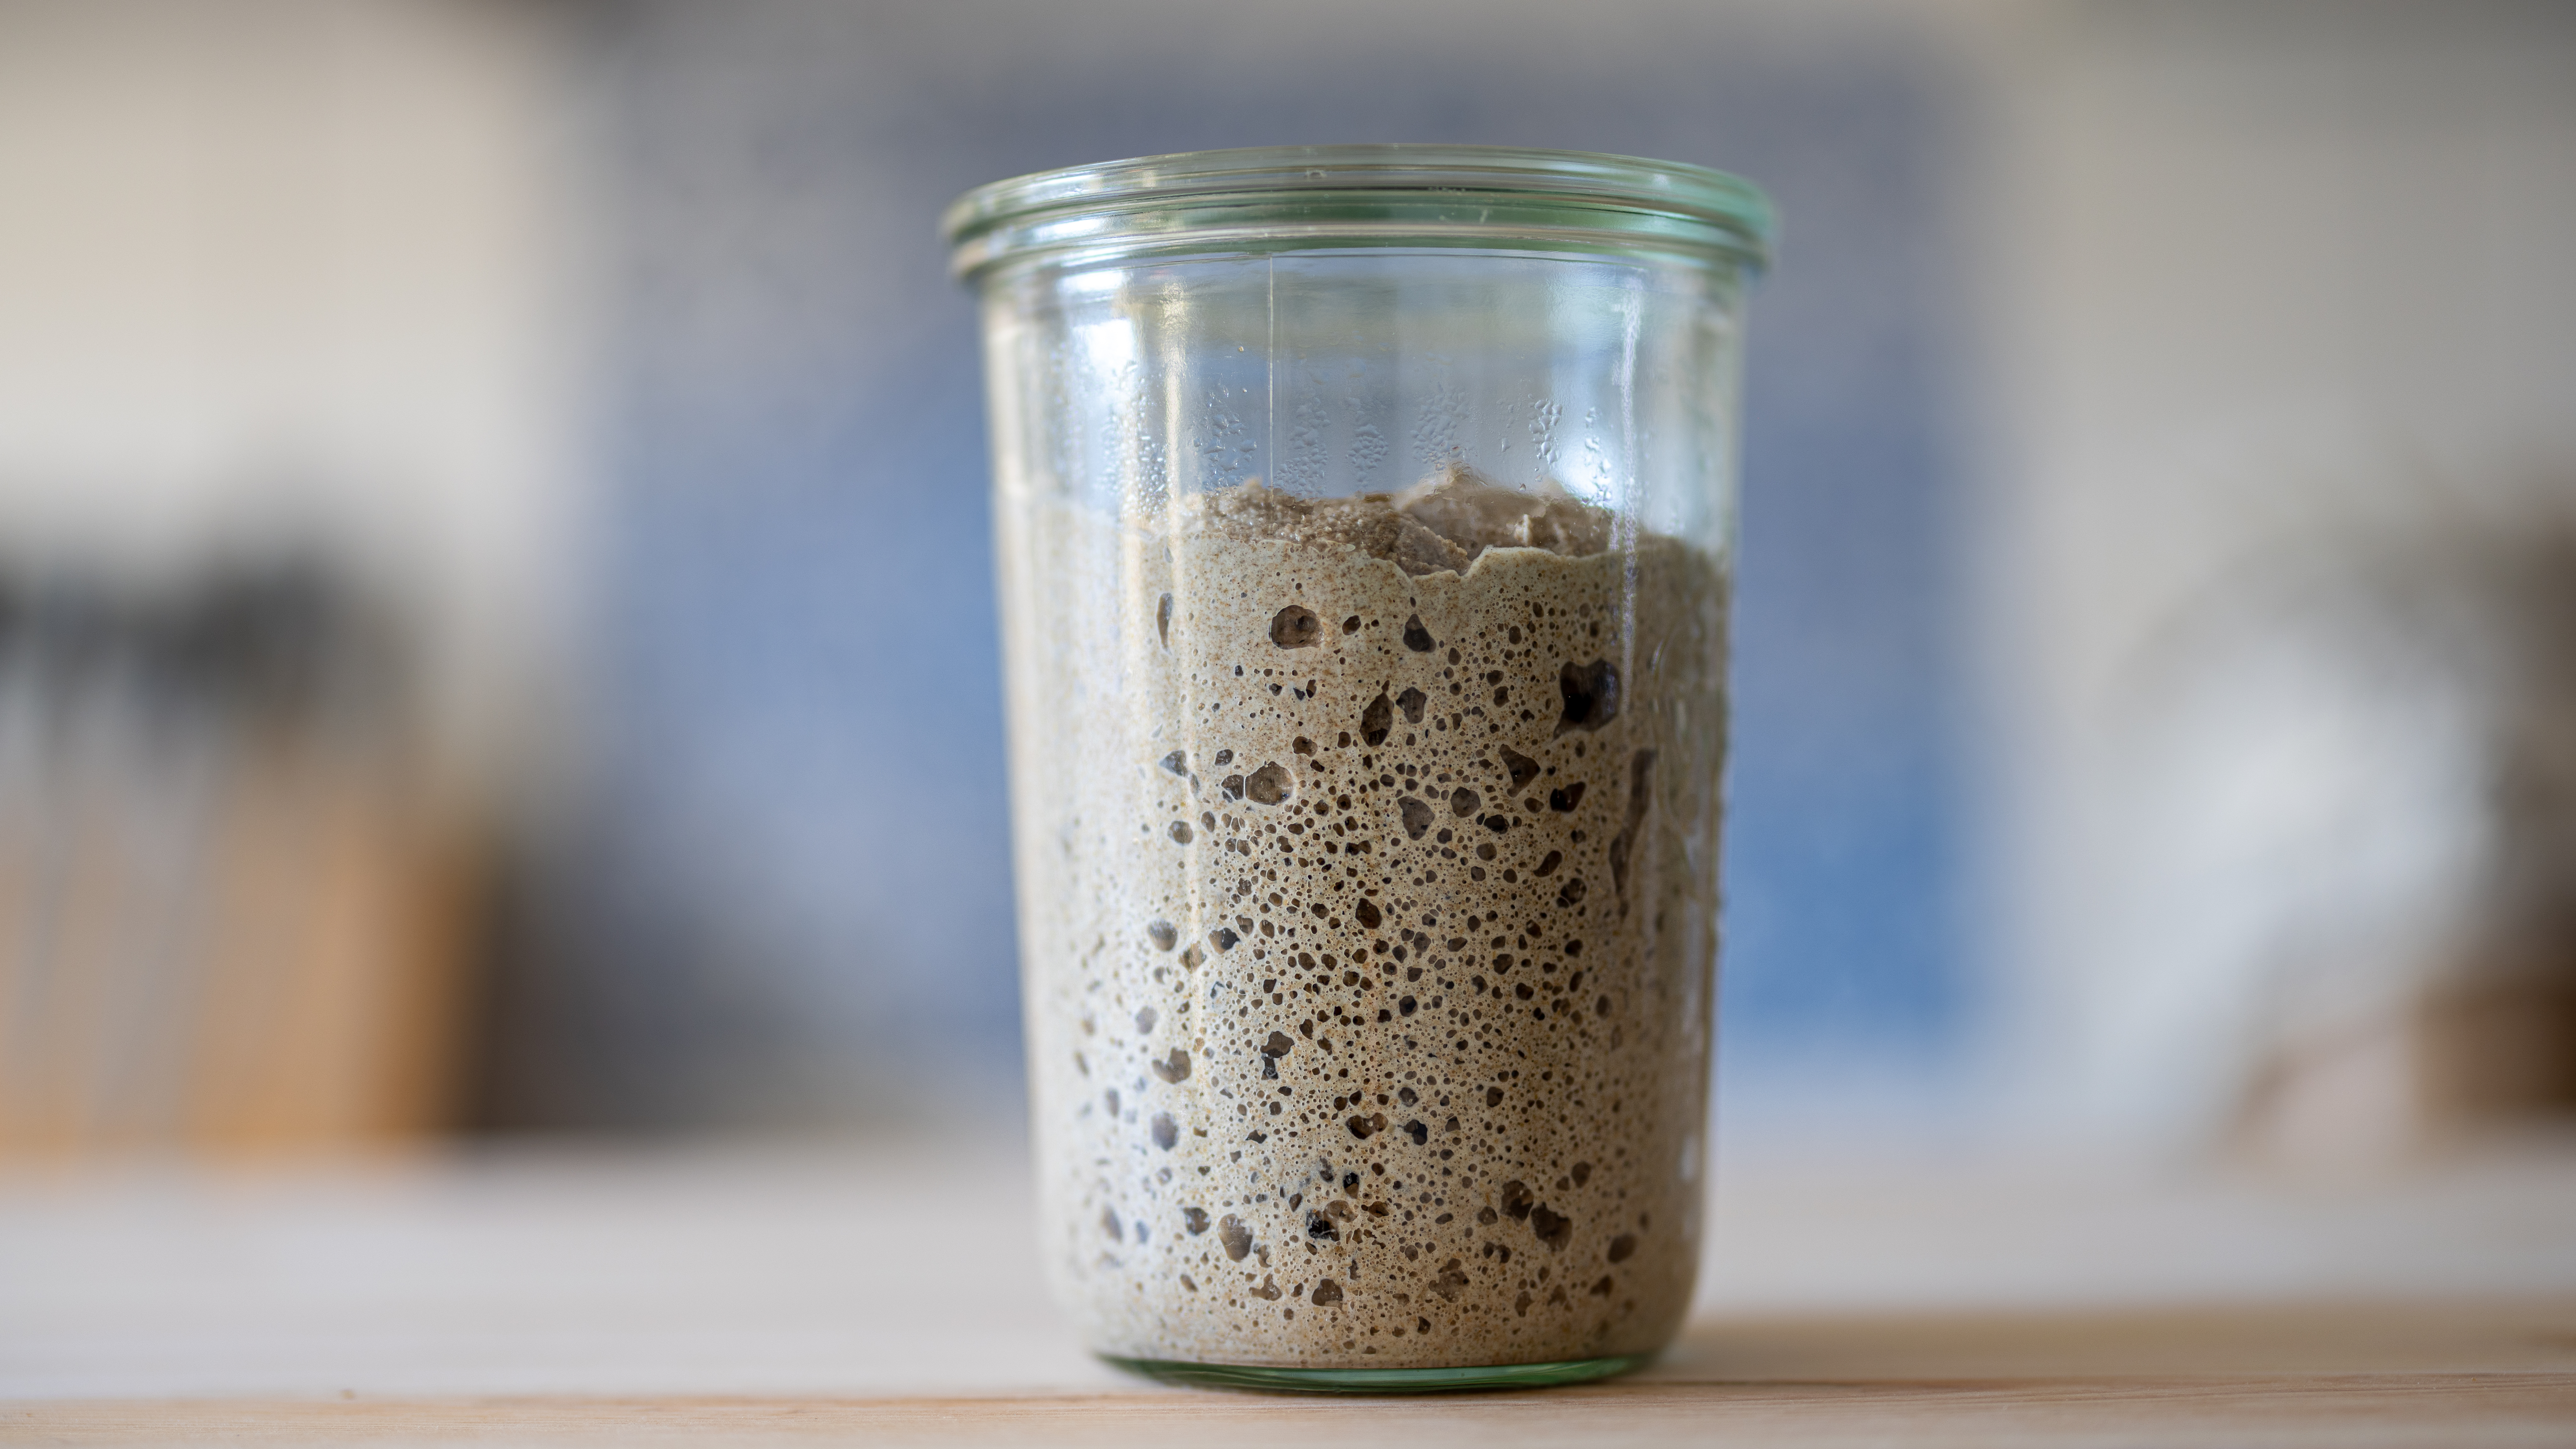
\includegraphics[width=\textwidth]{sourdough-starter.jpg}
  \caption{A very active sourdough starter shown by the bubbles in the dough}
  \label{fig:sourdough-starter}
\end{figure}

Making a sourdough starter is very easy. All you need
is a little bit of patience. The flour you should
use to setup your starter is ideally a whole flour.
You could use whole wheat, whole rye, whole spelt or
any other flour you have. In fact gluten free flours such
as rice or corn would also work. Don't worry, you can
change the flour later. Use whatever whole flour you
already have at hand.

Your flour is contaminated with millions of microbes. As explained
before in the chapter about wild yeast and bacteria, these
microbes live on the surface of the plant. That's why
a whole flour works better because you have more natural
contamination of the microbes you are trying to cultivate
in your starter. More of them live on the hull compared to the
endophytes living in the grain.

Simply weigh around 50 grams of flour and add another 50
grams of water. It doesn't have to be exactly 50 grams of both
water or flour. You could also use less and/or simply eyeball it.
The values are just shown as a reference. Don't use chlorinated
water to setup your starter. It should be bottled water ideally,
or here in Germany we can just use our tap water. Chlorine
is added to water to kill microorganisms. You will not
be able to grow a starter with chlorinated water. The hydration
of your dough is 100 percent. This means you have equal parts
of flour and water. Stir everything together so that all the flour
is properly hydrated. By adding water many of your microbes'
spores become activated. They exit hibernation mode and
become alive again. Cover your mixture with a lid. I like to
use a glass and place another inverted one on top. The container shouldn't
be airtight. You still want some gas exchange to be possible.

\begin{figure}[!htb]
  \includegraphics{figures/fig-starter-process.pdf}
  \caption{The process of making a sourdough starter from scratch}
  \label{fig:sourdough-starter-process}
\end{figure}

Now an epic battle begins. In one study scientists
have identified more than 150 different yeast species living
on a single leaf of a plant \cite{yeasts+biocontrol+agent}.
All of the different yeasts and bacteria are trying to get
the upper hand in this battle. Other pathogens such as mold
are also being activated as we added water. Only the strongest
most adaptable microorganisms will survive. By adding water to the
flour the starches start to degrade. The seedling tries to
sprout but it no longer can. Essential for this process is the
amylase enzyme. The compact starch is broken down to more
digestible sugars to fuel plant growth. Glucose is what the
plant needs in order to grow. The microorganisms that survive
this frenzy are adapted to consuming glucose. Luckily for us
bakers, the yeast and bacteria know very well how to metabolize
glucose. This is what they have been fed in the wild by the plants.
By forming patches on the leaf and protecting the plant from
pathogens they received glucose in return for their services.
Each of the microbes tries to defeat the other by consuming the
food fastest, producing agents to inhibit food uptake by others or by producing
bactericides and/or fungicides. This early stage of the starter
is very interesting as more research could possibly reveal
new fungicides or antibiotics. Depending on where your flour
is from, the starting microbes of your starter might be different
than the ones from another starter. Some people have also reported
how the microbes from your hand or air can influence your starter's
microorganisms. This makes sense to a certain extent. Your
hand's microbes might be good at fermenting your sweat, but
probably not so good and metabolizing glucose. The contamination
of your hands or air might play a minor role in the initial epic
battle. But only the fittest microbes fitting the sourdough's
niche are going to survive. This means the microorganisms that know
how to convert maltose or glucose will have the upper hand. Or the
microbes that ferment the waste of the other microbes. Ethanol created
by the yeast is metabolized by the bacteria in your sourdough. That's
why a sourdough has no alcohol. I can confirm the role of aerial
contamination to a certain extent. When setting up a new sourdough
starter the whole process is quite quick for me. After a few
days my new starter seems to be quite alive already. This might
be due to previous contamination of flour fermenting microbes in
my kitchen.

\begin{figure}[!htb]
  \includegraphics[width=\textwidth]{sourdough-starter-microbial-war}
  \caption{A simple visualization of the microbial warfare that happens during the making of a sourdough starter. The
  wild spores on the plant and flour become activated the moment flour and water is mixed.
  Only the most adapted flour-fermenting microbes will survive. Because of unwanted microbial fermentation it is advised
  to discard the feeding-leftovers of the first days. The surviving yeast and bacteria continuously try to
  outcompete each other for resources. New microbes have a hard time entering the starter and are eliminated.
  }
  \label{fig:sourdough-starter-microbial-war}
\end{figure}


Wait for around 24 hours and observe what happens to your starter.
You might see some early signs of fermentation already. Use your nose
to smell the dough. Look for bubbles in the dough. Your dough
might already have increased in size a little bit. Whatever
you see and notice is a sign of the first battle. Some microbes
have already been outperformed. Others have won the first battle.
After around 24 hours most of the starch has been broken down
and your microbes are hungry for additional sugars. With a spoon
take around 10 grams from the previous day's mixture and place
it in a new container. Again - you could also simply eye ball
all the quantities. It does not matter that much. Mix the 10
grams from the previous day with another 50 grams of flour
and 50 grams of water. Note the ratio of 1:5. I very often use
1 part of old culture with 5 parts of flour and 5 parts of water.
This is also very often the same ratio I use when making a dough.
A dough is nothing else than a sourdough starter with slightly different
properties. I'd always be using around 100-200 grams of starter
for around 1000 grams of flour (baker's math: 10-20 percent).
Homogenize your new mixture again with a spoon. Then cover
the mix again with a glass or a lid. If you notice the top of
your mixture dries out a lot consider using another cover. The
dried-out parts will be composted by more adapted microbes such as
mold. In many user reports, I saw mold being able to damage
the starter when the starter itself dried out a lot. You will
still have some mixture left from your first day. As this contains
possibly dangerous pathogens that have been activated we will discard
this mixture. Once your sourdough starter is mature never
discard it. It's long-fermented flour that is an excellent addon
used to make crackers, pancakes and or delicious hearty sandwich
bread. I also frequently dry it and use it as a rolling agent
for pizzas that I am making.

You should hopefully again see some bubbles, the starter increasing
in size and/or the starter changing its smell. Some people give
up after the second or third day. That is because the signs might no longer
be as dominant as they were on day one. The reason for this lies in only a few
select microbes starting to take over the whole sourdough starter. The most
adaptable ones are going to win. They are very small in quantity and will
grow in population with each subsequent feeding. Even if you see no signs
of activity directly, don't worry. There is activity in
your starter on a microscopic level.

24 hours later again we will repeat the same thing again until
we see that our sourdough starter is active. More on that in the
next section of this book.

\section{Determining starter readiness}

For some people the whole process of setting up a starter takes
only 4 days. For others it can take 7 days, for some even 20 days.
This depends on several factors including how good your wild microbes
are at fermenting flour. Generally speaking, with each feeding
your starter becomes more adapted to its environment. Your
starter will become better at fermenting flour. That's why
a very old and mature starter you receive from a friend might
be stronger than your own starter initially. Over time
your sourdough starter will catch up. Similarly, modern baking
yeast has been isolated like this from century old sourdough
starters.

\begin{figure}[!htb]
  \includegraphics{figures/fig-starter-readiness.pdf}
  \caption{A flow chart showing you how to determine if your sourdough starter is ready to be used.
  For checking readiness look at a size increase and take note of your starter's smell. Both are important
  indicators to check for readiness.}
  \label{fig:sourdough-starter-readiness}
\end{figure}

The key signs to look at are bubbles that you see in your starter
jar. This is a sign that the yeast is metabolizing your
dough and creates \ch{CO2}. The \ch{CO2} is trapped in your dough
matrix and then visualized on the edges of the container.
Also note the size increase of your dough. The amount the dough increases
in size is irrelevant. Some bakers claim it doubles, triples or quadruples.
The amount of size increase depends on your microbes, but also on
the flour that you use to make the starter. Wheat flour contains
more gluten and will thus result in a larger size increase. At
the same time the microbes are probably not more active compared
to when living in rye sourdough. You could only argue that
wheat microbes might be better at breaking down gluten compared
to rye microbes. That's one of the reasons why I decided to change
the flour of my sourdough starter quite often. I had hoped to create
an all-around starter that can ferment all sorts of different flour.\footnote
{Whether this is working I can't scientifically say.
Typically the microbes that have once taken place are very strong
and won't allow other microbes to enter. My starter has initially
been made with rye flour. So chances are that the majority of
my microorganisms are from a rye source.} Your nose is also
a great tool to determine starter readiness. Depending on
your starter's microbiome you should notice either the smell
of lactic acid or acetic acid. Lactic acid has dairy yogurty notes.
The acetic acid has very strong pungent vinegary notes. Some
describe the smell as glue or acetone. Combining the visual clues
of size increase and pockets plus the smell is the best way
to determine starter readiness.

In rare events your flour might be treated and prevent microbe growth.
This can happen if the flour is not organic and a lot of biochemical
agents have been used by the farmer. In that case simply try again
with different flour. 7 days is a good period of time to wait before
trying again.

Another methodology used by some bakers is the so called \emph{float test}.
The idea is to take a piece of your sourdough starter and place it
on top of some water. If the dough is full with gas it will float
on top of the water. If it's not ready, it can't float and will
sink to the bottom. This test does not work with every flour.
Rye flour for instance can't retain the gas as well as wheat flour
and thus in some cases will not float. That's why I personally
don't use this test and can't recommend it.

Once you see your starter is ready I would recommend giving it
one last feeding and then you are ready to make your dough in the
evening or the next day. For the instructions to make your
first dough please refer to the next chapters in this book.

If your first bread failed, chances are your fermentation hasn't
worked as expected. In many cases the source is your sourdough starter. Maybe
the balance of bacteria and yeast isn't optimal yet. In that case a good
solution is to keep feeding your starter once per day. With each feeding your
starter becomes better at fermenting flour. The microbes will adapt more and
more to the environment. Please also consider reading the stiff sourdough starter
chapter in this book. The stiff sourdough starter helps to boost the
yeast part of your sourdough and balance the fermentation.

\section{Maintenance}

\begin{figure}[!htb]
  \includegraphics{figures/fig-starter-maintenance.pdf}
  \caption{A full flowchart showing you how to conduct proper sourdough starter maintenance. You can use a
  piece of your dough as the next starter. You can also use left-over starter and feed it again. Choose an
  option that works best for your own schedule. The chart assumes that you are using a starter at a 100 percent
  hydration level. Adjust the water content accordingly when you use a stiff starter.}
  \label{fig:sourdough-maintenance-process}
\end{figure}

You have made your sourdough starter and your first bread. How do you perform
maintenance for your starter? There are countless of different maintenance
methods out there. Some people go completely crazy about their starter and
perform daily feedings of the starter. The key to understanding how to properly
conduct maintenance is to understand what happens to your starter after you
used it to make a dough. Whatever starter you have left, or a tiny piece of
your bread dough can serve to make your next starter.\footnote{I very often use all my
starter to make a dough. So if the recipe calls for 50g of starter I make
exactly 50g starter in advance. This means I have no starter left. In that
case I would proceed to take tiny bit of the dough at the end of the
fermentation period. This piece I would use to regrow my starter again.}


As explained earlier your starter is adapted
to fermenting flour. The microbes in your starter are very resilient. They
block external pathogens and other microbes. That is the reason why, when
buying a sourdough starter, you will preserve the original microbes. It is
likely that they are not going to change in your starter. They are outcompeting other
microbes when it comes to fermenting flour. Normally everything in nature
starts to decompose after a while. However, the microbes of your starter have
very strong defense mechanisms. In the end, your sourdough starter can be
compared to pickled food. Pickled food has been shown to stay good for a very
long period of time \cite{pickled+foods+expiration}. The acidity of your sourdough starter is quite
toxic to other microbes. The yeast and bacteria though have adapted to living
in the high-acid environment. Compare this to your stomach, the acidity
neutralizes many possible pathogens. As long as your starter has sufficient
food available it will outcompete other microbes. When the starter runs out of
food the microbes will start to sporulate. They prepare for a period of no
food and will then reactivate the moment new food is present. The
spores are very resilient and can survive under extreme conditions.
Scientists have claimed they found 250 million-year-old spores that are still
active \cite{old+spores}. While being spores
they are however more vulnerable to external pathogens such as mold.
Under ideal conditions though the spores can survive for a
long time.

But as long as they stay in the environment of your starter they live
in a very protected environment. Other fungi and bacteria have a hard time decomposing your left over starter mass.
I have seen only very few cases where the starter actually died. It is almost impossible
to kill a starter.

What happens though is that the balance of yeast and
bacteria changes in your starter. The bacteria is more fitted to living
in an acidic environment. This is a problem when you make another dough.
You want to have the proper balance of fluffiness and sour notes.
When a starter has hibernated for a long period, chances are that
you do not have a desirable balance of microbes.
Furthermore, depending on the time your starter hibernated you might only have
sporulated microbes left. So a couple of feedings will help to get your
sourdough starter into the right shape again.

The following are a couple of scenarios that will help you to conduct proper
starter maintenance, depending on when you want to bake the next time.

\textbf{I would like to bake again the next day:}

Simply take whatever starter you have left and feed it again. If you depleted
all your starter you can cut a piece of your dough. The dough itself is
nothing different than a gigantic starter. I recommend a 1:5:5 ratio like
mentioned before. So take 1 piece of starter, feed with 5 parts of flour and 5
parts of water. If it is very hot where you live, or if you want to make the
bread around 24 hours later after your last feeding, change the ratio. In that
case I would go for a 1:10:10 ratio. Sometimes I don't have enough starter.
Then I even use a ratio of 1:50:50 or 1:100:100. Depending on how much new
flour you feed it takes longer for your starter to be ready again.

\textbf{I would like to take a break and bake next week:}

Simply take your leftover starter and place it inside of your fridge. It will stay good
for a very long period. The only thing I see happening is the surface
drying out in the fridge. So I recommend drowning the starter in a little bit
of water. This extra layer of water provides good protection from the top
part drying out. As mold is aerobic it can not grow efficiently under
water \cite{mold+anaerobic}. Before using the starter again simply either stir
the liquid into the dough or drain it. If you drain the liquid you can use it
to make a lacto fermented hot sauce for instance.

The colder it is the longer you preserve a good balance of yeast and
bacteria. Generally, the warmer it is the faster the fermentation process is,
and the colder it is the slower the whole process becomes.
Below 4°C the starter fermentation almost completely stops. The
fermentation speed at low temperatures depends on the
strains of wild yeast and bacteria
that you have cultivated.

\textbf{I would like to take a several months break:}

Drying your starter might be the best option to preserve it in this case. As
you remove humidity and food your microbes will sporulate. As there is no
humidity the spores can resist other pathogens very well. A dried starter can
be good for years.

Simply take your starter and mix it with flour. Try to crumble the starter as
much as possible. Add more flour continuously until you notice that there is no
moisture left. Place the flour starter in a dry place in your house. Let it
dry out even more. If you have a dehydrator you can use this to speed up the
process. Set it to around 30°C and dry the starter for 12-20 hours. The next
day your starter has dried out a bit. It is in a vulnerable state as there is still a bit
of humidity left. Add some more flour to speed up the drying process. Repeat
for another 2 days until you feel that there is no humidity left. This is
important or else it might start to grow mold. Once this is done simply store the
starter in an airtight container. Or you can proceed and freeze
the dried starter. Both options work perfectly fine. Your sporulated starter
is now waiting for your next feeding. If available you can add some silica
bags to the container to further absorb excess moisture.

Initially, it would take 3 days or so for my starter to become alive again
after drying and reactivating it. If I do the same thing now my starter is
sometimes ready after a single feeding. It seems that the microbes adapt. The ones
that survive this shock become dominant subsequently.

So in conclusion the maintenance mode you choose depends on when you want to bake next.
The goal of each new feeding is to make sure your starter
has a desired balance of yeast and bacteria when making a dough. There is no need to provide your
starter with daily feedings, unless it is not mature yet. In that case, each
subsequent feeding will help to make your starter more adept at fermenting
flour.


\chapter{Sourdough starter types}
In this chapter of the book we will have a closer look
at different sourdough starter types and their respective
traits.

\begin{table}[htp!]
\centering
\resizebox{\textwidth}{!} & \textbf{Flour type}     & \multicolumn{1}{l|}{\textbf{Yeast activity}} & \textbf{Bacterial activity} \\ \hline
Regular               & 100                      & Strong wheat flour      & Balanced                                     & Balanced                    \\ \hline
Liquid                & 500                      & Very strong wheat flour & Minimal                                      & High                        \\ \hline
Stiff                 & 50-60                    & All wheat flour         & High                                         & Low                         \\ \hline
\end{tabular}%
}
\caption{\label{tab:starter-types-comparison}A comparison of different sourdough starter types}
\end{table}

Depending on the flour you have at hand the type of starter changes. With more
bacterial activity you have more gluten consumption of your microbes. So if
you want to bake a free standing loaf you need a flour with more gluten. The
more gluten you have the more of it can be broken down whilst still maintaining
dough integrity. If you live in a country where the climate to grow wheat
isn't ideal and you only have weaker flours, then a stiff sourdough starter
could be advised. The stiff sourdough starter will improve yeast activity and
reduce bacterial activity. If you are a chaser of a very sour bread and have a
very strong wheat flour then you can try to play with a liquid sourdough
starter. The key difference between all of the starters is how much water
is used in the starter. The regular starter having a 1:1 relationship of flour
to water. The liquid starter has a 5:1 water to flour ratio and the stiff
starter has half the flour as water.

You can change your starter type by just adjusting the feeding ratio of how
much flour and water you use. I frequently changed my starter type from
regular to liquid and then back to a stiff starter. After changing the
environment of your microbes apply feedings at the same ratio over a couple of
days so that they can adapt to the new environment. I could already see
changes after a single feeding, but I recommend 2 to 3 feedings, one feeding per
day to see a stronger effect.

Your dough is generally just a big sourdough starter. So your starter is going
to adapt and regrow inside of your main dough. But you can influence the
properties that your starter carries over to your main dough. If you have more
bacterial fermentation then your dough will also have slightly more bacterial
fermentation. If you have more yeast fermentation then your main dough will
have slightly more yeast fermentation. This is important to know when you are
working with a more mature unfed starter. Let's say your starter had last been
fed 48 hours ago, then chances are your bacteria is very active while the
yeast could be dormant. In such a case you can skip feeding your starter
before making another dough. Just use a very tiny amount of starter. For 1000g
of flour I would take around 10g of starter (1 percent in terms of baker's
math). If my starter is very young and had just been fed 6 to 8 hours ago I might
end up going up to 20 percent of starter. Remember that your dough is nothing
else other than a big starter. It will tremendously help you to figure out
your best next steps.

\section{Regular starter}

\begin{figure}[!htb]
  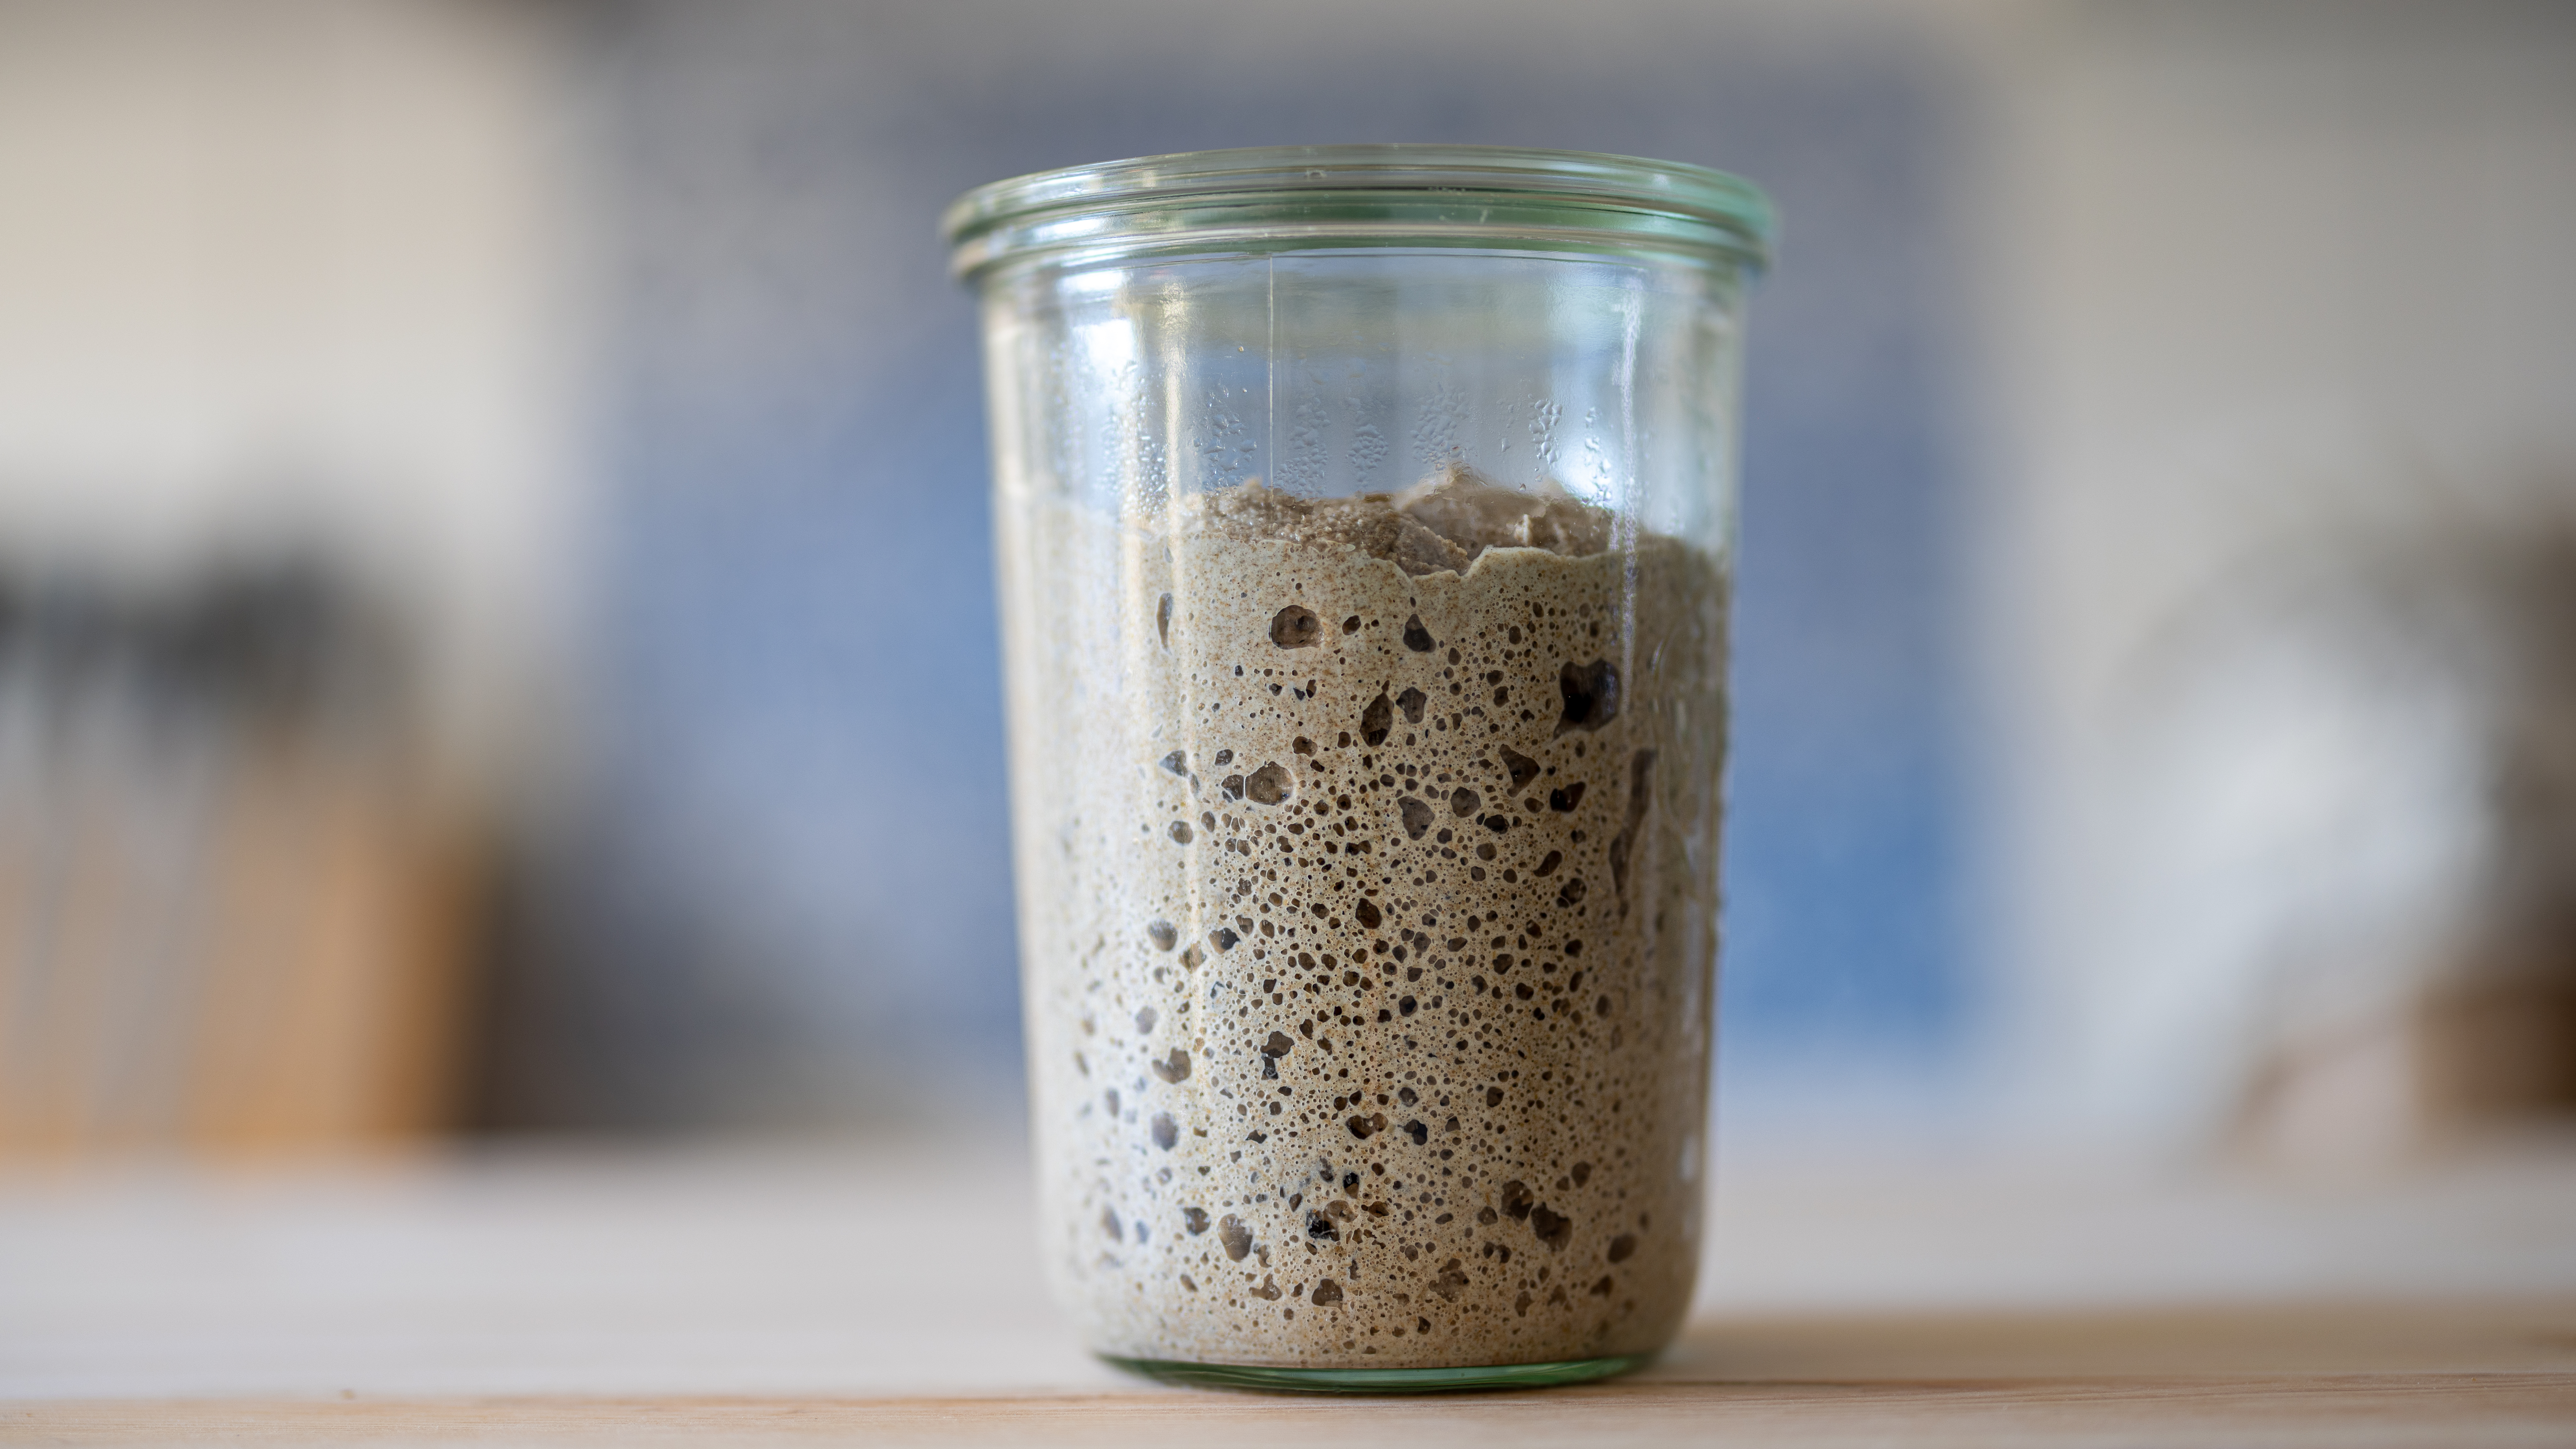
\includegraphics[width=\textwidth]{sourdough-starter.jpg}
  \caption{A regular sourdough starter at 100 percent hydration fed with rye flour}
  \label{fig:regular-sourdough-starter}
\end{figure}

The regular sourdough starter is made at a hydration of around 100 percent.
This means the starter has equal parts of flour and water. This is the most
common and must universal sourdough starter there is. The starter has a good
balance of yeast and bacteria. After a feeding the volume increases and
increases. After it reached a certain peak it will start to collapse again.

The best way to judge whether the starter is ready is to look at signs such as
pockets on the edges of your container. Also use the nose to to evaluate the
smell of your starter. If you feel that the starter doesn't perform in a
desirable way chances are that your yeast and bacteria ratios are off. In that
case frequently daily feedings using a 1:5:5 (starter:flour:water) ratio will
help.

The starter is perfect to use when utilizing stronger wheat or spelt flours.
It also nicely works with rye, emmer or einkorn. If you only have a weak flour
at hand with less gluten this starter might cause issue. As you tend to have
quite some bacterial activity gluten is going to be broken down fast. When
using the starter use around 1 to 20 percent starter based on the flour of your
dough.

Depending on the bacteria cultivated your starter either has a lactic (dairy),
a vinegary (acetic) or mix of both flavour profile. You can adjust your
starter's flavour by changing the type to a liquid starter.

\section{Liquid starter}

\begin{figure}[!htb]
  \centering
  \includegraphics[width=0.5\textwidth]{sourdough-starter-liquid.jpg}
  \caption{A liquid sourdough starter where the flour separates from the water. Bubbles indicate
  that is ready to be used.}
  \label{fig:liquid-sourdough-starter}
\end{figure}

The liquid starter is made at a hydration of around 500 percent. This means
the starter has way more water than flour. The additional layer of water on
top of the flour changes the microbiome of your starter.

By introducing this layer of water less oxygen is available throughout the
course of fermentation. This means that your starter will no longer be
producing acetic acid. The heterofermentative lactic acid bacteria will thrive
in this environment. This is a neat little trick to change your starter's
flavour profile from vinegary to lactic. Your starter is going to develop
dairy creamy notes. Interesting when changing the hydration again your starter
is going to maintain the liquid starter flavor profile, but then benefit again
from enhanced yeast activity. The liquid starter conversion is non reversible.
So ideally keep a backup of your starter before.

To commence with the
conversion simply take around 1 gram of your starter, mix with 5g flour and
25g water. Stir everything together properly. After a few minutes the flour is
going to start settling in at the bottom of your jar. Repeat this process over
a few days. Shake the starter gently to see if you can see tiny CO2 bubbles
moving in the liquid. This is a good sign that your starter is ready. Use your
nose to smell the starter. It should have a creamy dairy flavor note.

As you have more bacterial activity this starter works best with a very strong
flour that can withstand a long fermentation period. Using this starter with a
weak wheat flour will not work. If you do not care about baking a free
standing loaf then you can easily use this starter together with a loaf pan.
This starter also works great when making a hearty pancake dough. To use it I
shake the starter container until I see all ingredients are homogenized. Then
I use around 5 percent of it in terms of baker's math. So for 1000g of flour
that's around 50 grams of liquid starter. As it is very liquid you have to
include the 50 grams in your liquid calculation. I typically treat the starter
directly as liquid in the recipes. So if the recipe calls for 600 grams of water
and I use 50 grams of starter, then I would proceed and only use 550 grams of
water.

This type of starter is also an excellent mold combatant. As you are removing
oxygen from the equation aerobic mold can not properly grow. If your starter
has a mold problem then the liquid conversion could be the remedy. Take a
piece of your starter where you suspect no mold growth. Apply the conversion
as mentioned before. The mold will likely sporulate as it runs out of food.
With each new feeding you are reducing the mold spores. The spores can no
longe reactivate as they can not do so in the anaerobic conditions.

The liquid on top of your starter is an excellent resource that you could use
to make sauces. If you feel you would like to add a little bit of acidity,
drain the liquid part on your starter and use it. I have used it numerous
times to make lactofermented hot sauces.

\section{Stiff starter}
\label{section:stiff-starter}

\begin{figure}[!htb]
  \includegraphics[width=\textwidth]{sourdough-starter-stiff.jpg}
  \caption{A stiff sourdough starter that I used to make a Stollen dough for christmas. Note
  the bubbles on the edge of the container. The dough does not fall out of the jar.}
  \label{fig:stiff-sourdough-starter}
\end{figure}

The stiff starter is the driest of all the starters. It has a hydration of
around 50 to 60 percent. So for 100 grams of flour you are using around 60 to
60 grams of water.

In the stiffer environment the yeast thrives more. This means you will have
more CO2 production and less acid production. In my tests this is a game
changer especially if you are using weaker gluten flours. The wheat flours in
my home country Germany tend to be lower in gluten. For wheat to build gluten warm conditions
are preferred (SOURCE NEEDED). When following recipes from other bakers I
could never achieve similar results. When following timings my doughs would
simply collapse and become super sticky. Only when I started to buy more
expensive wheat flour my results started to change. As not everyone can afford
these special baking flours and due their limited availability I stumbled upon the
stiff sourdough starter. I made several tests where I used the same amount of
starter and flour. I only changed the hydration between all the starters. I
would then proceed and place a balloon on top of each of the jars. The stiff
starter jar was clearly inflated the most. On place 2 the regular starter
followed. On place three the liquid starter followed with way less CO2
production.

\begin{figure}[!htb]
  \includegraphics[width=\textwidth]{stollen}
  \caption{A German christmas stollen made with a stiff starter instead of yeast}
  \label{fig:stollen}
\end{figure}

I then proceeded and bought a cheap low cake flour in my nearby supermarket.
This flour before had caused me massive headache before. I made a sourdough bread
exactly how I would normally do. I had to reduce the hydration a bit as a low
gluten flour does not soak up as much water. Then I replaced the starter with
the stiff starter. The dough felt amazing and was suddenly able to withstand a
much longer fermentation period. The bread had great oven spring and tasted
very mild. I am still yet to find a proper explanation why the yeast part of
the dough is more active. Maybe it is not. It could also be that the bacteria
is inhibited by the lack of water.

When making the stiff sourdough starter start with using around 50 percent
water. If you are using a whole wheat flour, or a strong flour consider going
up to 60 percent. All the ingredients should mix together very well. There
should be no crumbly flour left. This is a common mistake I have seen when
people tried to make the stiff starter. Yes it should be dry, but not to a
point where it is a brick of cement. If you ever made a pasta dough, this is
exactly the same way how the dough should feel like.

To evaluate whether your stiff starter is ready look for a dome. Also look for
pockets of air on the edges of your container. Use your nose to smell the
starter. It should have a mild smell. It also tends to smell way more
alcoholic than the other starters.

When using the starter use around 1 to 20 percent depending on the ripeness of
your starter. In summer times I typically use around 10 percent and in winter
times around 20 percent. This way you can also control the fermentation speed.
Mixing the starter can be a little bit annoying as it hardly homogenises with
the rest of the dough. In this case you can try to dissolve the starter in the
water you are about to use for your dough. This will make mixing a lot easier.


\section{Lievito madre or pasta madre}

The Lievito madre also known as pasta madre belongs to the same category as
the stiff sourdough starter. After conducting hours of research I could not
find a difference in pasta madre and lievito madre. Both of terms seem to be
used interchangeably in literature.

In many recipes this starter is made directly
from dried or fresh fruits. You can make a starter also from leaves from your
garden. As described before the wild yeast and bacteria consume the glucose
from the plants leaves. All the options work. When making a starter directly
from dried fruits you sometimes lack the bacterial part of the fermentation.
The acidity is very important in order to clean your starter from possible
pathogens. If you decide to make your starter from fruits make sure it also
acidifies properly when making a dough. A tool such as a pH meter can be of
optimal help. Generally the lower the pH the higher the acidity. The acidity
should be below 4.2 to know that your starter produces sufficient acidity.

Some bakers cleanse the lievito madre in a bath of water. This is supposed to
remove excess acidity. In my own experiments I have not been able to confirm
this methodology. The acidity remains the same. The only reason this could
make sense is if you also tried to boost anaerobic microorganisms. However then the
starter would need to remain in this environment for quite some time and not just
a few hours.

Baking with sourdough is simple. It's just flour and water. When seeing a recipe
from an experienced baker you wonder, wait, that's it? There is nothing more
to it? I feel that this might be the reason why some bakers have so complicated
feeding procedures. They resort to several feedings per day at a certain given ratio.
This makes the baker feel a little more elitist. Of course over time as
more and more people follow this procedure it becomes a self fulfilling prophecy.
The more experienced you become the higher the chances are that a bogus starter
feeding guide will reward you with beautiful results. The reason however is
not in the starter routine. The reason is that you better understand the fermentation
and become better at reading the signs of your dough.

If I had one starter type to choose I would go for the stiff starter. In many cases
it will provide you with consistent great results with little effort.
In my experience you can make any yeast based dough and just replace
the yeast directly with the stiff sourdough starter. You will be able
to achieve even better results with the stiff starter.

Lastly no matter which starter type you choose, you can control how sour
you want your dough to be. The longer you push the fermentation the more
acidity is going to be piled up. The only difference is that for a given
volume increase the stiff starter will produce the least acidity. So for a
volume increase of 100 percent, the liquid starter has produced most acidity,
followed by the regular starter and then the stiff starter. If you wait long
enough the stiff starter will have produced the same amount of acidity as the
other starters. But before doing so it also has produced a lot more CO2. If
you like the sour flavour you have to push your fermentation longer. This also
means you either need to bake in a loaf pan or have a very strong gluten flour
that is able to withstand long fermentation times.


\chapter{Flour types}
\chapter{Flour types}%
\label{ch:flour-types}
\begin{quoting}
In this chapter we will have a closer look at different flour types
and their respective categorization. We will also look at common
ways to distinguish different flours of the same type, this way you can more
confidently purchase the flour you need.
\end{quoting}

The most basic flour type is a whole grain flour, in this case the whole seed has
been grounded to smaller pieces. Sometimes, depending on what you want to bake,
the hearty taste of the bran might not be desired. In this case you can use
whiter flours. Together with sieves, mills remove larger parts of the seed's
hull.  The seed already contains a pre-built germ from the plant waiting to be
activated. The whitest flour you can get is mostly just the starch part of the seed.
Depending on which layers are still present, different names are used to describe the
type of flour.

\begin{table}[!htb]
    \centering
        \documentclass[tikz]{standalone}
\usepackage{tikz}

\definecolor{codeblue}{RGB}{69, 161, 248}
\definecolor{codegray}{RGB}{40, 40, 40}
\usetikzlibrary{shapes,arrows}
\tikzstyle{decision} = [diamond, draw, fill=codegray, text=white,
    text width=4.5em, text badly centered, node distance=3cm, inner sep=0pt]
\tikzstyle{block} = [rectangle, draw, fill=codeblue,  text=white,
    text width=5em, text centered, rounded corners, minimum height=4em]
\tikzstyle{line} = [draw, -latex']


\begin{document}
\begin{tabular}{llrrr}
\toprule
\textbf{USA}      & \textbf{UK}      & \multicolumn{1}{l}{\textbf{Germany}}      & \multicolumn{1}{l}{\textbf{France}}      & \multicolumn{1}{l}{\textbf{Italy}} \\ \midrule
Cake              & Soft flour       & T405                                       & T45                                       & 00                                       \\ \midrule
All purpose       & Plain flour      & T550                                       & T55                                       & 0                                        \\ \midrule
                  &                  & T812                                       & T80                                       & 1                                        \\ \midrule
                  &                  & T1050                                      & T110                                      & 2                                        \\ \midrule
Whole             & Whole            & Vollkorn
                  & T150                                      & Integrale
                  \\ \bottomrule
\end{tabular}
\end{document}

        \caption[Labelling of wheat flour]{A comparison of how different types
            of wheat flour are labelled in different countries.}%
        \label{tab:flour-types-comparison}
\end{table}

In Germany, the ash content is used to describe the flours. The lab will burn
\qty{100}{\gram} of flour in the oven. Then afterwards the remaining ash is extracted
and measured. Depending on the quantity the flour is categorized. If the flour
is of type 405, then \qty{405}{\mg} of ash have remained after burning the
flour. The more hull parts the flour has, the more minerals remain, therefore the
higher the number, the closer the flour is to whole flour. The numbers are
slightly different between each grain type. Generally though, the higher the
value, the heartier the taste is going to be.

\begin{figure}[htb!]
  \includegraphics[width=\textwidth]{wheat-kernel-overview}
  \caption[Content of a wheat kernel]{An overview of a wheat kernel together
      with its content~\cite{wheat+kernel}.}%
  \label{fig:wheat-kernel-overview}
\end{figure}

If you compare different grain types, there are grains with high gluten, low gluten
and no gluten. Gluten is what enables bread to have its fluffy consistency.
Without gluten the baked goods wouldn't have the same properties. Managing
gluten makes the whole bread-making process more complex as more steps are involved.

A dough without gluten doesn't have to be kneaded as the role of kneading is
to create
the gluten bonds. The more you knead, the stronger they become. With low-gluten
and no-gluten flours, you only have to mix the ingredients together, making
sure you properly homogenize everything.

During fermentation
the gluten degrades as the microorganisms metabolize it. When too much gluten
has been converted your dough will no longer have the wheat-like structure previously
described. For no/low gluten flour your main focus is managing acidity, you do not
want the final bread to be too sour. Conversely you do not have to worry about
the gluten degradation, removing a huge headache from the equation.

\begin{table}[!htb]
    \centering
        \begin{tabular}{@{}>{\bfseries}lcccc@{}}
\toprule
\thead{Grain type}        & \thead{Homogenize} & \thead{Knead} & \thead{Stretch \& Fold} & \thead{Shape} \\ \midrule
Wheat                     & Yes & Yes & Yes & Yes \\ 
\textgreater{}~70\% Wheat & Yes & Yes & Yes & Yes \\ 
Spelt                     & Yes & Yes & Yes & Yes \\ 
Rye                       & Yes & No  & No  & No  \\ 
Emmer                     & Yes & No  & No  & No  \\ 
Einkorn                   & Yes & No  & No  & No  \\ 
Rice                      & Yes & No  & No  & No  \\ 
Corn                      & Yes & No  & No  & No  \\ \bottomrule
\end{tabular}

        \caption[Different types of grain]{An overview of different grain
          types and the steps involved in the respective bread making process.}
\end{table}

Because gluten has a special role, the rest of this chapter is dedicated to having a
closer look at different gluten flours and how to distinguish them. Like wheat
spelt contains significant amounts of gluten, so the same characteristics hold
true.

Several recipes call for wheat bread flour, but bread flour can refer to different types
of flour. It could be a T405 or a T550 in Germany---this is very often
classified incorrectly---the terms \emph{strong} or \emph{bread} flour in this case
refer to the properties of the flour. A bread flour is considered to have a
higher amount of protein and thus gluten. This flour is excellent when you
want to make a sourdough bread as your dough allows for a longer leavening
period. As described earlier, the gluten is consumed by your microorganisms.
The more gluten you have, the longer your dough keeps its integrity. If you wanted
to make a cake, you might want to use a flour with less gluten. The gluten binding
properties might not be desirable since the final cake could have a chewy texture.

In conclusion, not every T405, T45 or T00 flour is the same. Depending on the properties
of the plant they come from, the flours will have different properties. For that reason
some countries like Germany have introduced additional scales to evaluate the quality of the
wheat. The category \emph{A} refers to good quality wheat that can be blended
with poorer qualities to improve the flour. The category \emph{B} refers to
average wheat that can be used to create different baked goods. Category \emph{C}
is used for wheat that has poor baking qualities. This could happen, for instance,
if the wheat already started to sprout and thus lost some of its desirable
baking properties. This type of wheat is typically used in animal feed or
as fermentable biomass for generators. Category \emph{E} refers to \emph{Elite} wheat. It's
the highest quality of wheat. This kind of wheat can only be harvested when the
wheat has grown under optimal conditions. You can compare this to a winery
that uses only the best grapes to make a reserve wine. Unfortunately, this is
usually not printed
on the packaging of the flour that you buy. You can look out for the protein
value as a possible indicator. However, large mills blend flours together to
maintain quality throughout the years. Blended flour is also not listed on
the packaging. It might be that bakeries extract gluten from some flour and
then mix it in order to create better baking flours.

In Italy the so-called
\emph{W-value} has been introduced to better show how the flour will behave.
A dough is made, and then the resistance of this dough to kneading is measured.
The more gluten a flour has, the more elastic the dough is, and the more it will
resist kneading. A higher W flour will have a higher gluten content and allow for a longer
fermentation period. But at the same time, it is also harder for the microbes to
inflate the dough as there is more balloon material. To make an excellent fermented
product out of a high W flour you will need to have a long fermentation period.
The long fermentation period also means that your microbes will enrich
your dough with more flavor.

\begin{table}[!htb]
    \centering
        \begin{tabular}{@{}rcll@{}}
\toprule
\thead{W-Value} & \thead{Hydration (\%)} & \thead{Uses} & \thead{Fermentation time} \\ \midrule
0--150          & 50     & Cookies             & Very short\\ 
150--250        & 50--60 & Cakes, Bread, Pizza & Short-Medium\\ 
250--350        & 60--70 & Bread, Pizza        & Long      \\ 
350+            & 70--90 & Bread, Pizza        & Very long \\ \bottomrule
\end{tabular}

        \caption[Fermentation time versus W-value]{An overview of different
            levels of W-values and the respective hydrations and fermentation
            times.}%
        \label{tab:w-value}
\end{table}

Generally, when aiming to
bake free standing sourdough bread, aim for a higher protein content. If the
gluten value is relatively low, your bread will collapse faster. Baking bread
is still possible, but it might be easier to use other techniques such as a
loaf pan, to consider skillet bread or flatbread.

An additional, rarely considered characteristic of good flour is the level of damage to the
starch molecules. This is a common problem when you are trying to mill your own wheat flours at
home. The chances are that your home mill is not able to achieve the same results
a larger mill can. The damaging of the starches is essential to improve the
properties of the dough. You will have better gelatinization and water
absorption with properly damaged starch~\cite{starch+damage+flour}. As more
starch is damaged, the surface area increases. This improves how water interacts with the flour.
This also provides a larger surface that your microbes can use to attack the molecules
and start the fermentation process.

I~am still
yet to find a good way of milling my own wheat flour at home. Even after trying to
mill the flour 10~times with short breaks, I~was not able to achieve the same
properties as with commercially milled flour. The doughs I~would make felt
good, maybe a bit coarse. However, during baking the doughs would start to
de-gas quickly and turn into very flat breads. I~have had great success though when
utilizing home-milled flour together with a loaf pan or as a pan bread. If you
have found great ways to work with home-milled flour, please reach out. The potential
of using home-milled flours is huge. It would enable even distant communities
to grow their own wheat and be able to produce amazing freshly baked bread.


\chapter{Bread types}
\chapter{Bread types}%
\label{ch:bread-types}
\begin{quoting}
In this chapter you will learn about different bread types and their
advantages and disadvantages.  You can also find very simple recipes for
flatbread and pan loaf.  The former is probably the most accessible, least
effort type of bread you can make, while the latter is a little more involved.
Free standing bread has its own chapter, due to its increased complexity.
\end{quoting}

\section{Introduction}%
\label{sec:intro}

In this section we classify bread by its baking techniques. The appearance and
taste will of course be different, but you can get excellent bread with each
of them. Some breads will require investment and technique, as depicted in
Table~\ref{tab:bread-types-comparison}.  Flatbread is probably the most
accessible, least effort type of bread you can make. If you are a busy person
and/or don’t have an oven, this might be exactly the type of bread you should
consider. 
\begin{table}[!htb]
    \centering
        \documentclass[tikz]{standalone}
\usepackage{tikz}

\definecolor{codeblue}{RGB}{69, 161, 248}
\definecolor{codegray}{RGB}{40, 40, 40}
\usetikzlibrary{shapes,arrows}
\tikzstyle{decision} = [diamond, draw, fill=codegray, text=white,
    text width=4.5em, text badly centered, node distance=3cm, inner sep=0pt]
\tikzstyle{block} = [rectangle, draw, fill=codeblue,  text=white,
    text width=5em, text centered, rounded corners, minimum height=4em]
\tikzstyle{line} = [draw, -latex']


\begin{document}
\begin{tabular}{llll}
\toprule
                                 & \textbf{Flatbread}  & \textbf{Loaf pan bread} & \textbf{Free standing bread} \\ \midrule
\textbf{Cooking method}          & Fire, pan, barbecue & Oven                    & Oven                         \\ \midrule
\textbf{Working time in minutes} & 3                   & 5                       & 60                           \\ \midrule
\textbf{Flour types}             & All                 & All                     & Gluten flours                \\ \midrule
\textbf{Difficulty}              & Very easy           & Easy                    & Difficult                    \\ \midrule
\textbf{Cost}                    & Low                 & Medium
                                 & High                         \\ \bottomrule
\end{tabular}
\end{document}

        \caption[Different bread types]{An overview of different bread types
            and their respective complexity.}%
        \label{tab:bread-types-comparison}
\end{table}

\section{Flatbread}%
\label{sec:flatbread}

Flatbread is probably the simplest sourdough bread to make.
To make a flatbread no oven is required; all you need is a stove.

\begin{figure}[!htb]
  \includegraphics[width=\textwidth]{flat-breads-selection}
  \caption[Flatbread selection with different flours]{An assorted selection of
      different flatbreads made with sourdough. From left to right:
      Wheat~tortilla, rye, spelt and corn.}%
\end{figure}

This type of bread is super simple to make as you can skip
a lot of the technique that is normally required to make wheat doughs.
The flatbread can be made with all kinds of flours. You can even use
flour without gluten, such as corn or rice flour, to make the
dough. To make the flatbread a little more fluffy, you
can use a little bit of wheat flour. The developing gluten
will trap the gases. During baking, these gases will
inflate the dough.

Another trick to improve the texture of the flatbread is to
make a very wet dough. A lot of the water will evaporate
during the baking process and thus make the bread fluffier.
If your water content is very high, it will produce a
pancake-like consistency, as you can see in
Table~\ref{tab:flat-bread-ingredients}

\begin{table}[!htb]
    \centering
        \documentclass[tikz]{standalone}
\usepackage{tikz}

\definecolor{codeblue}{RGB}{69, 161, 248}
\definecolor{codegray}{RGB}{40, 40, 40}
\usetikzlibrary{shapes,arrows}
\tikzstyle{decision} = [diamond, draw, fill=codegray, text=white,
    text width=4.5em, text badly centered, node distance=3cm, inner sep=0pt]
\tikzstyle{block} = [rectangle, draw, fill=codeblue,  text=white,
    text width=5em, text centered, rounded corners, minimum height=4em]
\tikzstyle{line} = [draw, -latex']


\begin{document}
\begin{tabular}{lll}
\toprule
                           & \textbf{Flat breads} & \textbf{Pancakes}                        \\ \midrule
\textbf{Flour}             & 100g                               & 100g                       \\ \midrule
\textbf{Water}             & 100g (100\%)                       & 300g (300\%)               \\ \midrule
\textbf{Sourdough starter} & 5-20g (5-20\%)                     & 5-20g (5-20\%)             \\ \midrule
\textbf{Salt}              & 2g (2\%)                           & 2g (2\%)                   \\ \midrule
\textbf{When bake?}        & Dough increased 50 percent in size & Bubbles
visible on surface \\ \bottomrule
\end{tabular}
\end{document}

        \caption[Flatbread recipe]{Flatbread or pancake recipe for 1 person.
            Multiply the ingredients to increase portion size.  Refer to the
            Section~\ref{section:bakers-math}
            ``\nameref{section:bakers-math}'' to learn how to understand and
            use the percentages properly.}%
            \label{tab:flat-bread-ingredients}
\end{table}

For a full recipe including the process of making such a flatbread,   refer to
Subsection~\ref{subsec:flat-bread-recipe}

\subsection{Flatbread framework}%
\label{subsec:flat-bread-framework}

As explained above, if you are just getting started, making a flatbread is the
easiest way to start making great bread at home. With just a
few steps, you can stop buying bread forever. This works with
any flour, including gluten-free options.

\begin{flowchart}[!htb]
\centering
  \begin{tikzpicture}[node distance = 3cm, auto, every node/.style={inner sep=10, outer sep=0}]
\node [start] (init) {Mix ingredients};
  \node [block, right of=init, node distance=5cm] (wait) {Wait for dough to be ready};
  \node [success, right of=wait, node distance=5cm] (bake_bread) {Bake bread on stove};
  \path [line] (init) -- (wait);
  \path [line] (wait) -- (bake_bread);
\end{tikzpicture}

  \caption[The process to make a sourdough flatbread]{The process of making a flatbread is very
      simple, requiring very little effort. This type of bread is especially
      handy for busy bakers.}%
  \label{fig:flat-bread-process}
\end{flowchart}

This is my go-to recipe that I~use to make bread whenever
I~have little time or when I~am abroad. You can choose
between two options:
%
\begin{enumerate}
    \item A flatbread similar to a roti or naan bread
    \item Sourdough pancakes.
\end{enumerate}

To get started prepare your sourdough starter. If it has not been used for a very
long time, consider giving it another feed. To do so, simply take \qty{1}{\gram} of your
existing sourdough starter and feed it with \qty{5}{\gram} of flour and \qty{5}{\gram} of water.
If you do this in the morning, your sourdough starter will be ready in the evening. The
warmer it is, the sooner it will be ready,  consider
using warm water if it is very cold where you live.

\begin{figure}[htb!]
\centering
  \includegraphics[width=1.0\textwidth]{flat-bread-wheat}
  \caption[Wheat flatbread]{A flatbread made with purely wheat flour. The
      dough is drier at around \qty{60}{\percent} hydration. The drier dough
      is a little harder to mix. As wheat contains more gluten, the dough
      puffs up during the baking process.}
\end{figure}

This way you should have around \qty{11}{\gram} of sourdough ready in the evening. You will have
the perfect quantity to make a dough for one person. In case you want to make more
bread, simply multiply the quantities shown in
Table~\ref{tab:flat-bread-ingredients}.

Then in the evening simply mix the ingredients as shown in the table. Your dough
is going to be ready in the morning. It's typically ready after 6--12~hours. If
you use more sourdough starter it will be ready faster, conversely it will take
longer if you use less. Try to aim for a fermentation time of 8--12~hours as
by using your dough too soon, the flavor might not be as good. By using your
dough later it might become a little more sour. The best option is to
experiment and see what you personally like the most.

After mixing the ingredients together cover the container, this prevents the
dough from drying out and makes
sure no fruit flies get access. A transparent container will be helpful
when getting started. You can observe the dough more easily and see when
it is ready.

\begin{figure}[htb]
\centering
  \includegraphics[width=1.0\textwidth]{ethiopian-woman-checking-bread}
  \caption[Ethiopian \emph{injera}]{An Ethiopian woman baking an \emph{injera}
      made using teff flour.  The image has been provided by Charliefleurene
      via Wikipedia.}
\end{figure}

If you used the flatbread option with less water, look at the size increase
of your dough. It should have increased at least \qty{50}{\percent} in size.
Also look out for bubbles on the sides of your container.

When using the pancake recipe, look out for bubbles on the surface of your dough.
In both cases use your nose to check the scent of your dough. Depending
on your sourdough starter's microbiome your dough will have
dairy, fruity, alcoholic notes or vinegary, acetic notes. Relying
on the smell of your dough is the best way to judge whether your
dough is ready or not. Timings are not reliable as they
depend on your starter and the temperature. If your dough
is ready too soon, you can now move it directly to the fridge and bake
it at a later, more convenient time. The low temperature will halt the fermentation
process\footnote{There are some exceptions. In some rare cases your starter
might also work at lower temperatures. You might have cultivated microbes that work best at
low temperatures. Nevertheless, fermentation
is always slower the colder it gets. A fridge really helps to preserve the state
of your dough.}
and your dough will last for several days. The longer you wait, the more sour the
bread is going to be. The fridge is a great option in case you want to
take the dough with you when visiting friends. People are going
to love you for the freshly baked flatbreads or pancakes. If you dare,
you can also taste a little bit of your raw uncooked dough. It is likely
going to taste relatively sour. I~do this frequently to better evaluate the
state of my doughs.

\begin{figure}[!htb]
\centering
  \includegraphics[width=1.0\textwidth]{injera-pancake-texture.jpg}
  \caption[Teff sourdough pancake]{A sourdough pancake made with teff flour.
      The pockets come from evaporated water and \ch{CO2} created by the
      microbes.  The image has been provided by Łukasz Nowak via Wikipedia.}
\end{figure}

If you are feeling lazy or don't have time, you could also use older sourdough starter
to make the dough directly without any prior starter feedings. Your sourdough starter
is going to regrow inside your dough. Remember that the
final bread might be a bit more on the sour side as the balance of yeast to
bacteria could be off. In the Table~\ref{tab:flat-bread-ingredients}
I~recommended using around \qtyrange{5}{20}{\percent}
of sourdough starter based on the flour to make the dough. If you were to follow
this approach, just use around \qty{1}{\percent} and make the dough directly.
The dough is probably going to be ready 24~hours later, depending on the temperature.

If you want to make sweet pancakes, add some sugar and optional eggs to your dough
now. A good quantity of eggs is around one~egg per \qty{100}{\gram} of flour.
Stir your dough a little bit and it will be ready to be used. You'll
have delicious sweet savory pancakes, the perfect combination. By
adding the sugar now, you make sure that the microbes don't have
enough time to fully ferment it. If you had added the sugar
earlier, no sweet flavor would be left  12~hours later.

To bake your dough heat your stove to medium temperature. Add a little bit of
oil to the pan. This helps with heat distribution and ensures even cooking.
With a spatula or a spoon place your dough in the pan. If your dough
was sitting in the fridge, bake it directly. There is no need to wait for your
dough to come to room temperature. If you have a lid,
place it on your pan. The lid helps to cook your dough from the top.
The evaporating water will circulate and heat up the dough's surface. When
making a flatbread, make the dough around \qty{1}{\cm} thick. When using the
pancake option, opt for around \qtyrange{0.1}{0.5}{\cm} depending on what you
like.

\begin{figure}[htb]
\centering
  \includegraphics[width=1.0\textwidth]{einkorn-crumb.jpg}
  \caption[Einkorn crum]{The crumb of a flatbread made with einkorn as flour.
      Einkorn is very low in gluten and thus does not trap as much \ch{CO2} as
      a wheat based dough. To make the dough fluffier use more water or
      consider adding more wheat to the mix of your dough.}
\end{figure}

After 2--4~minutes flip over the pancake or flatbread. Bake it for the same
time from the other side. Depending on what you like, you can wait a little
longer to allow the bread to become a bit charred. The longer you
bake your bread, the more of the acidity is going to evaporate. If your
dough is a bit more on the sour side, you can use this trick to balance
out the acidity. This really depends on which flavor you are looking for.

When making a flatbread I~recommend wrapping the baked flatbreads in a kitchen
towel. This way more of the evaporating humidity stays inside of your bread,
making sure your flatbreads stay nice and fluffy for a longer period after the
bake. A similar strategy is used when making corn tortillas.

You can safely store the baked flatbreads or pancakes in your fridge
for weeks. When storing make sure to store them in an airtight plastic bag so that
they do not dry out. If they dry out, spray them with some water and toast them.
They will be almost as good as when they were freshly baked.

Keep a little bit of your unbaked dough. You can use it to make the next
batch of bread or pancakes for the next day. If you want to bake a few days later, add
a little bit of water and flour and store this mixture in your fridge
for as long as you like\footnote{The starter will stay good for months. If you expect to
leave it longer, consider drying a little bit of your sourdough starter.}.

\subsection{Simple flatbread recipe}%
\label{subsec:flat-bread-recipe}

By following the steps outlined in this section,
you'll be introduced to a versatile bread that's perfect for a myriad of
culinary applications. Whether you're scooping up a savory dip,
wrapping a flavorful filling, or simply enjoying a piece with a drizzle
of olive oil, these flatbreads are sure to impress.

\subsubsection*{Ingredients}
\begin{tabular}{r@{}rl@{}}
\qty{400}{\gram} &~(\qty{100}{\percent}) & Flour (wheat, rye, corn, whatever
                                            you have at hand)\\
\qty{320}{\gram} &  (\qty{80}{\percent}) & Water, preferably at room
                                            temperature\\
\qty{80}{\gram}  &  (\qty{20}{\percent}) & Active sourdough starter\\
\qty{8}{\gram}   &   (\qty{2}{\percent}) & Salt\\
\end{tabular}

\subsubsection*{Instructions}
\begin{description}
\item[Prepare the dough] In a large mixing bowl, combine the flour and water.
    Mix until you have a shaggy dough with no dry spots.

    Add the sourdough starter and salt to the mixture. Incorporate them
    thoroughly until you achieve a smooth and homogenized dough.

\item[Fermentation:] Cover the bowl with a lid or plastic wrap. Allow the dough
    to rest and ferment until it has increased by at least \qty{50}{\percent}
    in size.  Depending on the temperature and activity of your starter, this
    can take anywhere from 4 to 24~hours.

\item[Cooking preparation:] Once the dough has risen, heat a pan over medium
    heat.  Lightly oil the pan, ensuring to wipe away any excess oil with a
    paper towel.

\item[Shaping and cooking:] With a ladle or your hands, scoop out a portion of
    the dough and place it onto the hot pan, spreading it gently like a
    pancake.

    Cover the pan with a lid. This traps the steam and ensures even cooking
    from the top, allowing for easier flipping later.

    After about 5~minutes, or when the bottom of the flatbread has a
    golden-brown crust, carefully flip it using a spatula.

    \emph{Adjusting cook time.} If the flatbread appears too dark, remember to
    reduce the cooking time slightly for the next one.  Conversely, if it's
    too pale, allow it to cook a bit longer before flipping.

    Cook the flipped side for an additional 5~minutes or until it's also
    golden brown.

\item[Storing:] Once cooked, remove the flatbread from the pan and place it on
    a kitchen towel. Wrapping the breads in the towel will help retain their
    softness and prevent them from becoming overly crisp.  Repeat the cooking
    process for the remaining dough.

\item[Serving suggestion:] Enjoy your sourdough flatbreads warm, paired with
    your favorite dips, spreads, or as a side to any meal.

\end{description}


\section{Loaf pan bread}%
\label{sec:loaf-pan-bread}

Loaf pan bread is made using the help of a special loaf pan
or loaf tin. The edges of the pan provide additional support
for the dough to rise. Making a bread using a loaf pan requires
an oven.

\begin{figure}[!htb]
  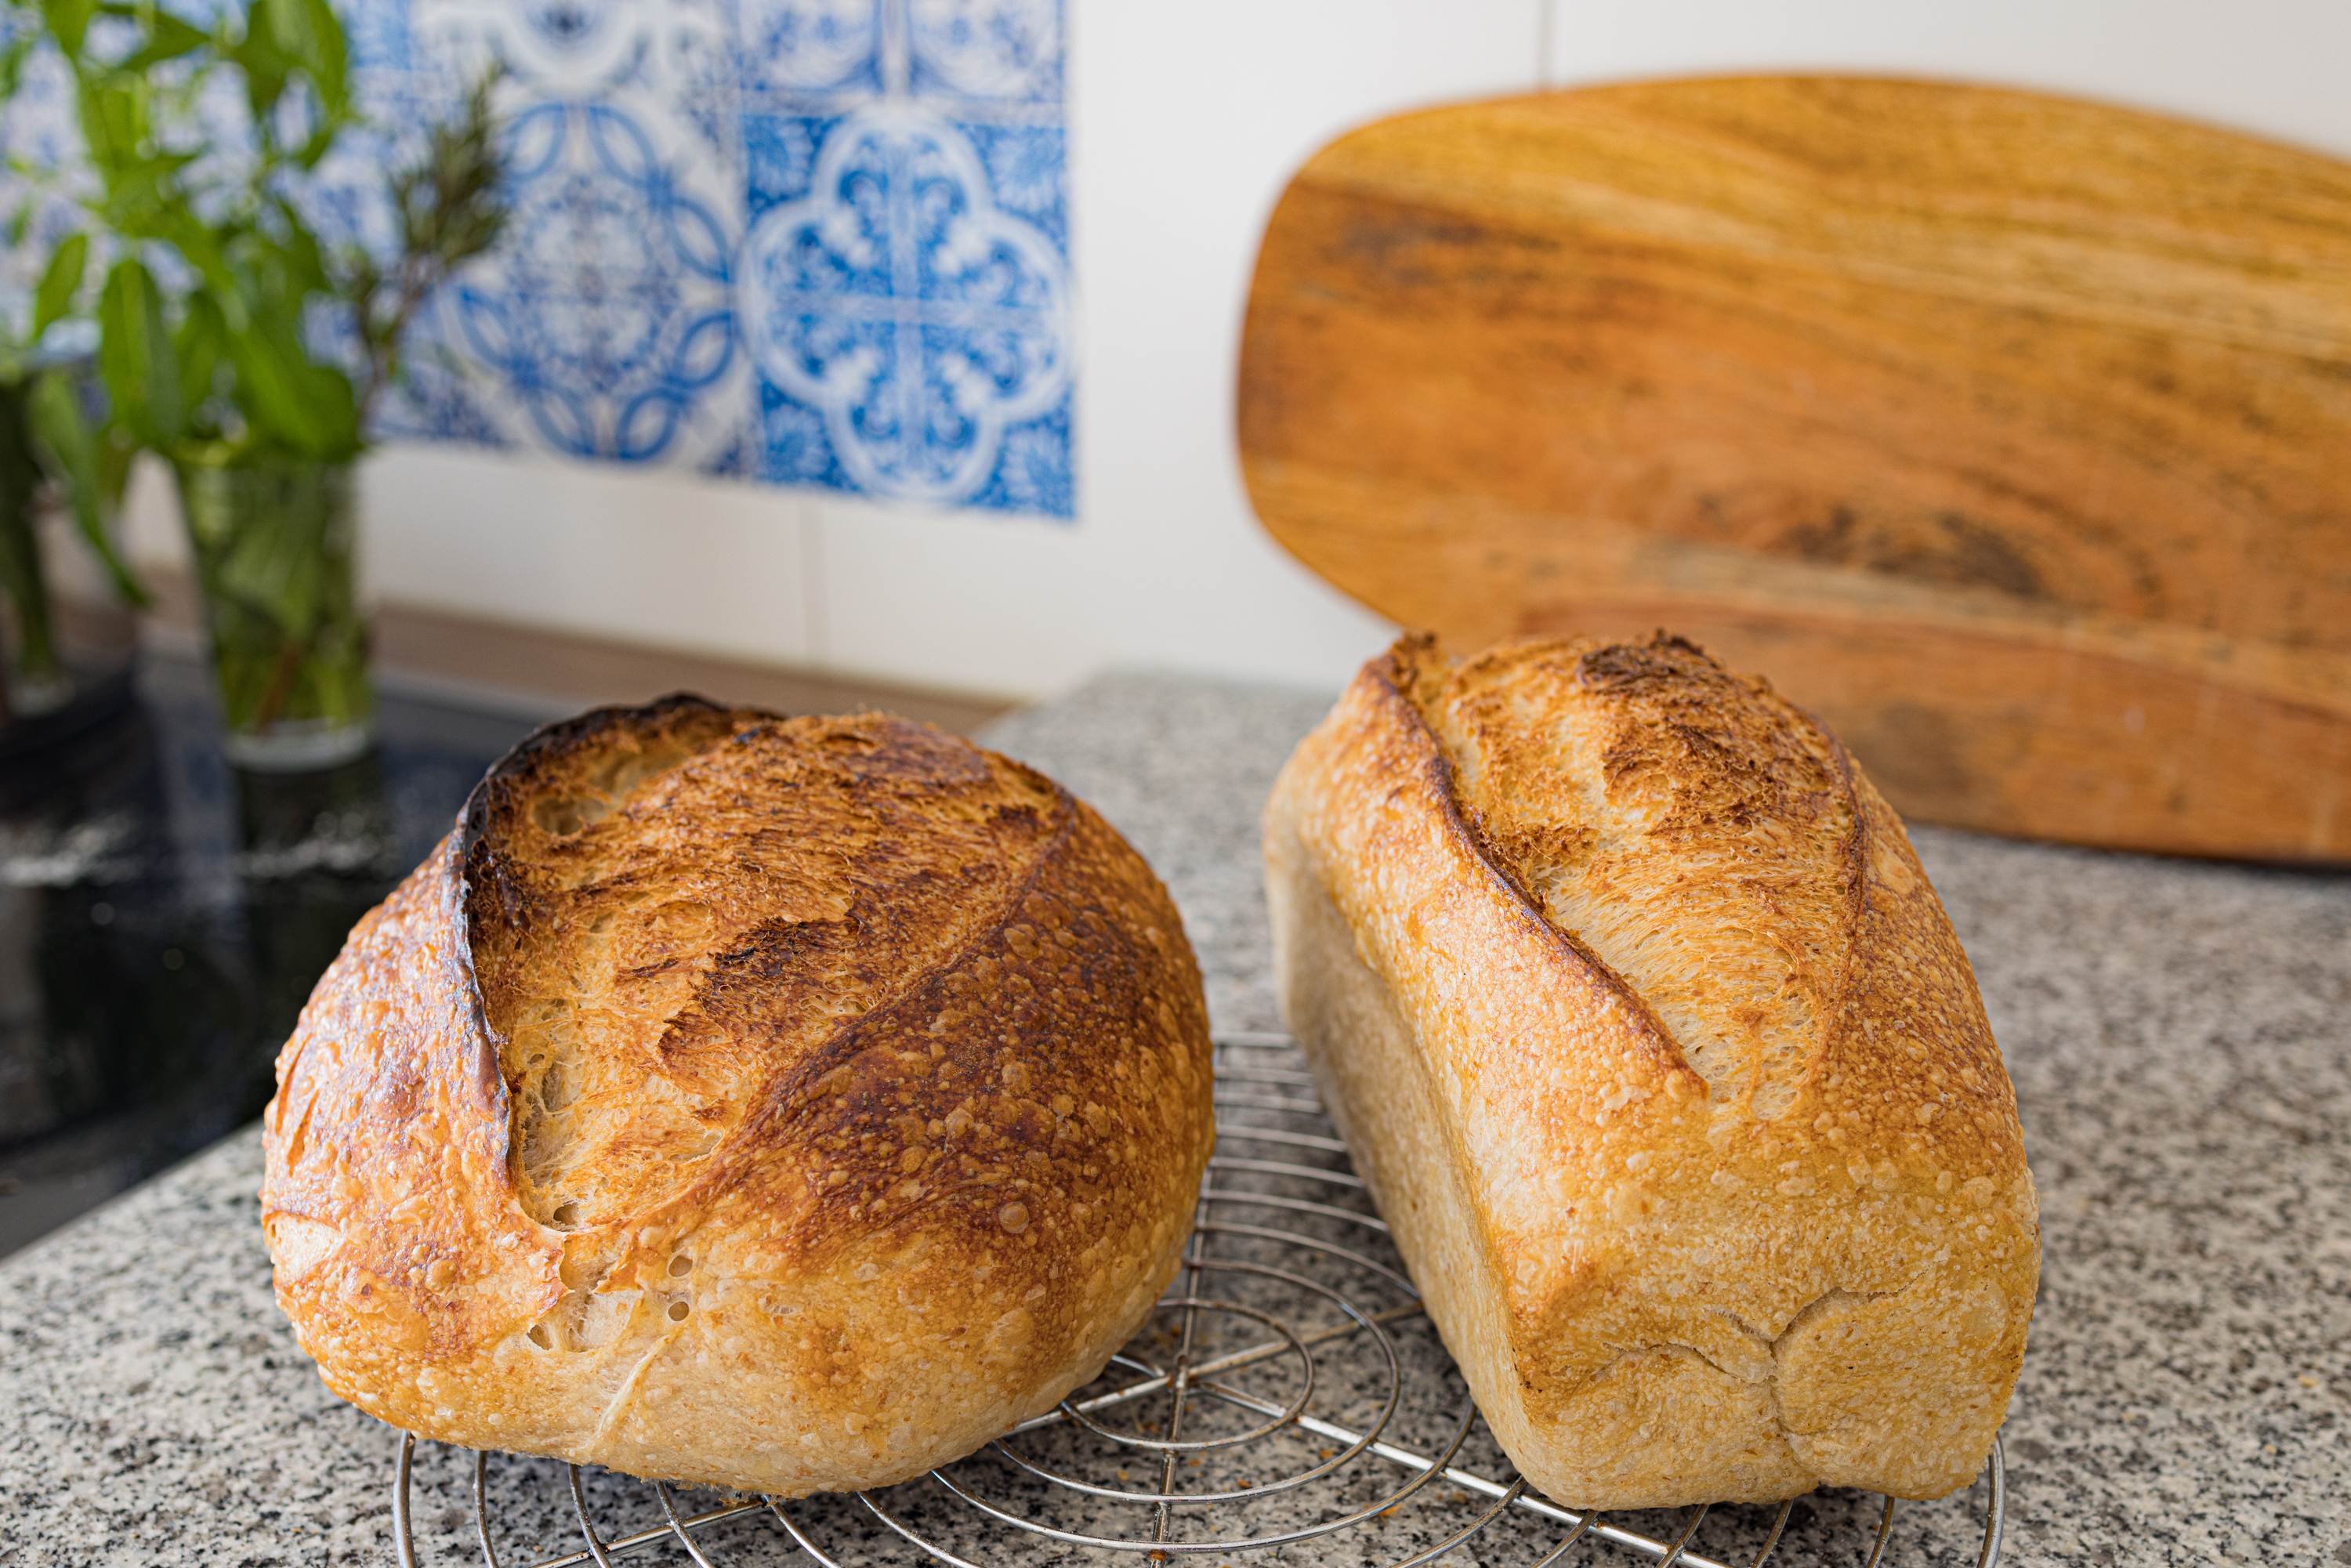
\includegraphics[width=\textwidth]{loaf-pan-free-standing.jpg}
  \caption[Freestanding bread and pan bread]{A freestanding bread and a wheat
      loaf pan bread. Both of them received a small incision before baking
      which helps to control how they open up.}%
  \label{fig:free-standing-loaf-pan}
\end{figure}

After mixing your dough, you can place it directly into the loaf pan.
This makes the whole process simpler since you can skip steps such
as shaping the dough.

To make a great loaf pan bread with little work:

\begin{enumerate}
    \item Mix the ingredients of your dough (gluten free works too)
    \item Place into the loaf pan
    \item Wait until your dough has roughly doubled in size
    \item Bake in a non pre-heated oven for around 30--50~minutes
\end{enumerate}

Knowing the exact baking time is sometimes a little challenging
as it might be that the outside of your bread is cooked but
the inside is still raw. The best way is to use a thermometer
and measure the core temperature. At around  \qty{92}{\degreeCelsius}
(\qty{197}{\degF}) your dough is done. I~generally bake loaf pan bread at
around  \qty{200}{\degreeCelsius} (\qty{390}{\degF}), which is a little less
than my freestanding bread which I~bake at  \qty{230}{\degreeCelsius}
(\qty{445}{\degF}). That's because it takes a while for the dough
to bake properly inside the loaf pan. The edges don't heat up
as quickly. Then the top part of the dough is properly cooked, while
the inside isn't yet. When baking make sure to use steam
or simply place another equally sized loaf pan on top
of your loaf pan. This way you simulate a Dutch oven. The dough's
evaporating moisture will stay inside.

A good trick to make excellent loaf pan bread is to make a very
sticky dough. You can opt for a hydration of \qtyrange{90}{100}{\percent}, almost
resembling a default sourdough starter. Just like with flatbread,
the high humidity helps to make a more airy, fluffy crumb. The bread will
also be a bit chewier. This type of bread made with rye is my family's favorite
style of bread.  The hearty rye flavor paired with the sticky consistency really
makes an excellent sandwich bread.

To improve the structure you can also consider using around \qty{50}{\percent}
wheat flour in your mix. The gluten network will develop as your
dough ferments and allow for more gas to be trapped in the dough.

A common problem you will face when making a loaf pan bread is
the dough sticking to the pan. Use a generous amount of oil to grease
your pan. A nonstick vegetable oil spray can do wonders.
Don't clean your loaf pans with soap. Just use a kitchen towel
to clean them. With each bake a better patina forms, making your
pan more and more stick resistant.

What's amazing about this type of bread is that it works
with every flour. The overall time to work the dough is probably
less than 5~minutes, making it very easy to integrate
into your daily routine. Furthermore, loaf pans use the space
in your oven very efficiently. Using pans I~can
easily bake 5 loaves at the same time in my home oven.
Normally I~would need multiple baking sessions for
freestanding loaves.

\section{Free standing bread}

A freestanding loaf is baked entirely without supporting
baking vessels in your oven. To make a freestanding loaf more steps
and tools are required.

\begin{figure}[!htb]
\centering
  \includegraphics[width=1.0\textwidth]{free-standing-loaf.jpg}
  \caption[Freestanding sourdough bread]{A freestanding sourdough bread. Note
      the incision known as an \emph{ear} and the oven spring clearly
      distinguish this type of bread from flatbread and loaf pan bread.}
\end{figure}

When using wheat, make sure to mix your dough enough to develop a gluten network.
Allow the dough to reach a certain size increase during the fermentation.
Afterward, divide and pre-shape the dough into the desired visual shape you
would like. Each shape requires a different technique. Sometimes achieving
the right shape can be challenging. Making a baguette, for instance,
requires performing more steps. Mastering this technique takes several attempts.

Once the dough is shaped, it is proofed again for a certain
period of time. Once the dough is ready, a sharp tool such
as a razor blade is used to make an incision into the dough.
This helps control how the dough opens up during the baking process.

All these steps require practice. Each of them has to be
performed perfectly, without mistakes.
But after baking you will be rewarded with a beautiful bread
with great taste and consistency.

There is a dedicated recipe and tutorial for this type of bread in the
\nameref{chapter:wheat-sourdough} chapter.


\chapter{Wheat sourdough}
\label{chapter:wheat-sourdough}
In this chapter, you will learn how to make
free-standing wheat sourdough bread.

\begin{figure}[!htb]
  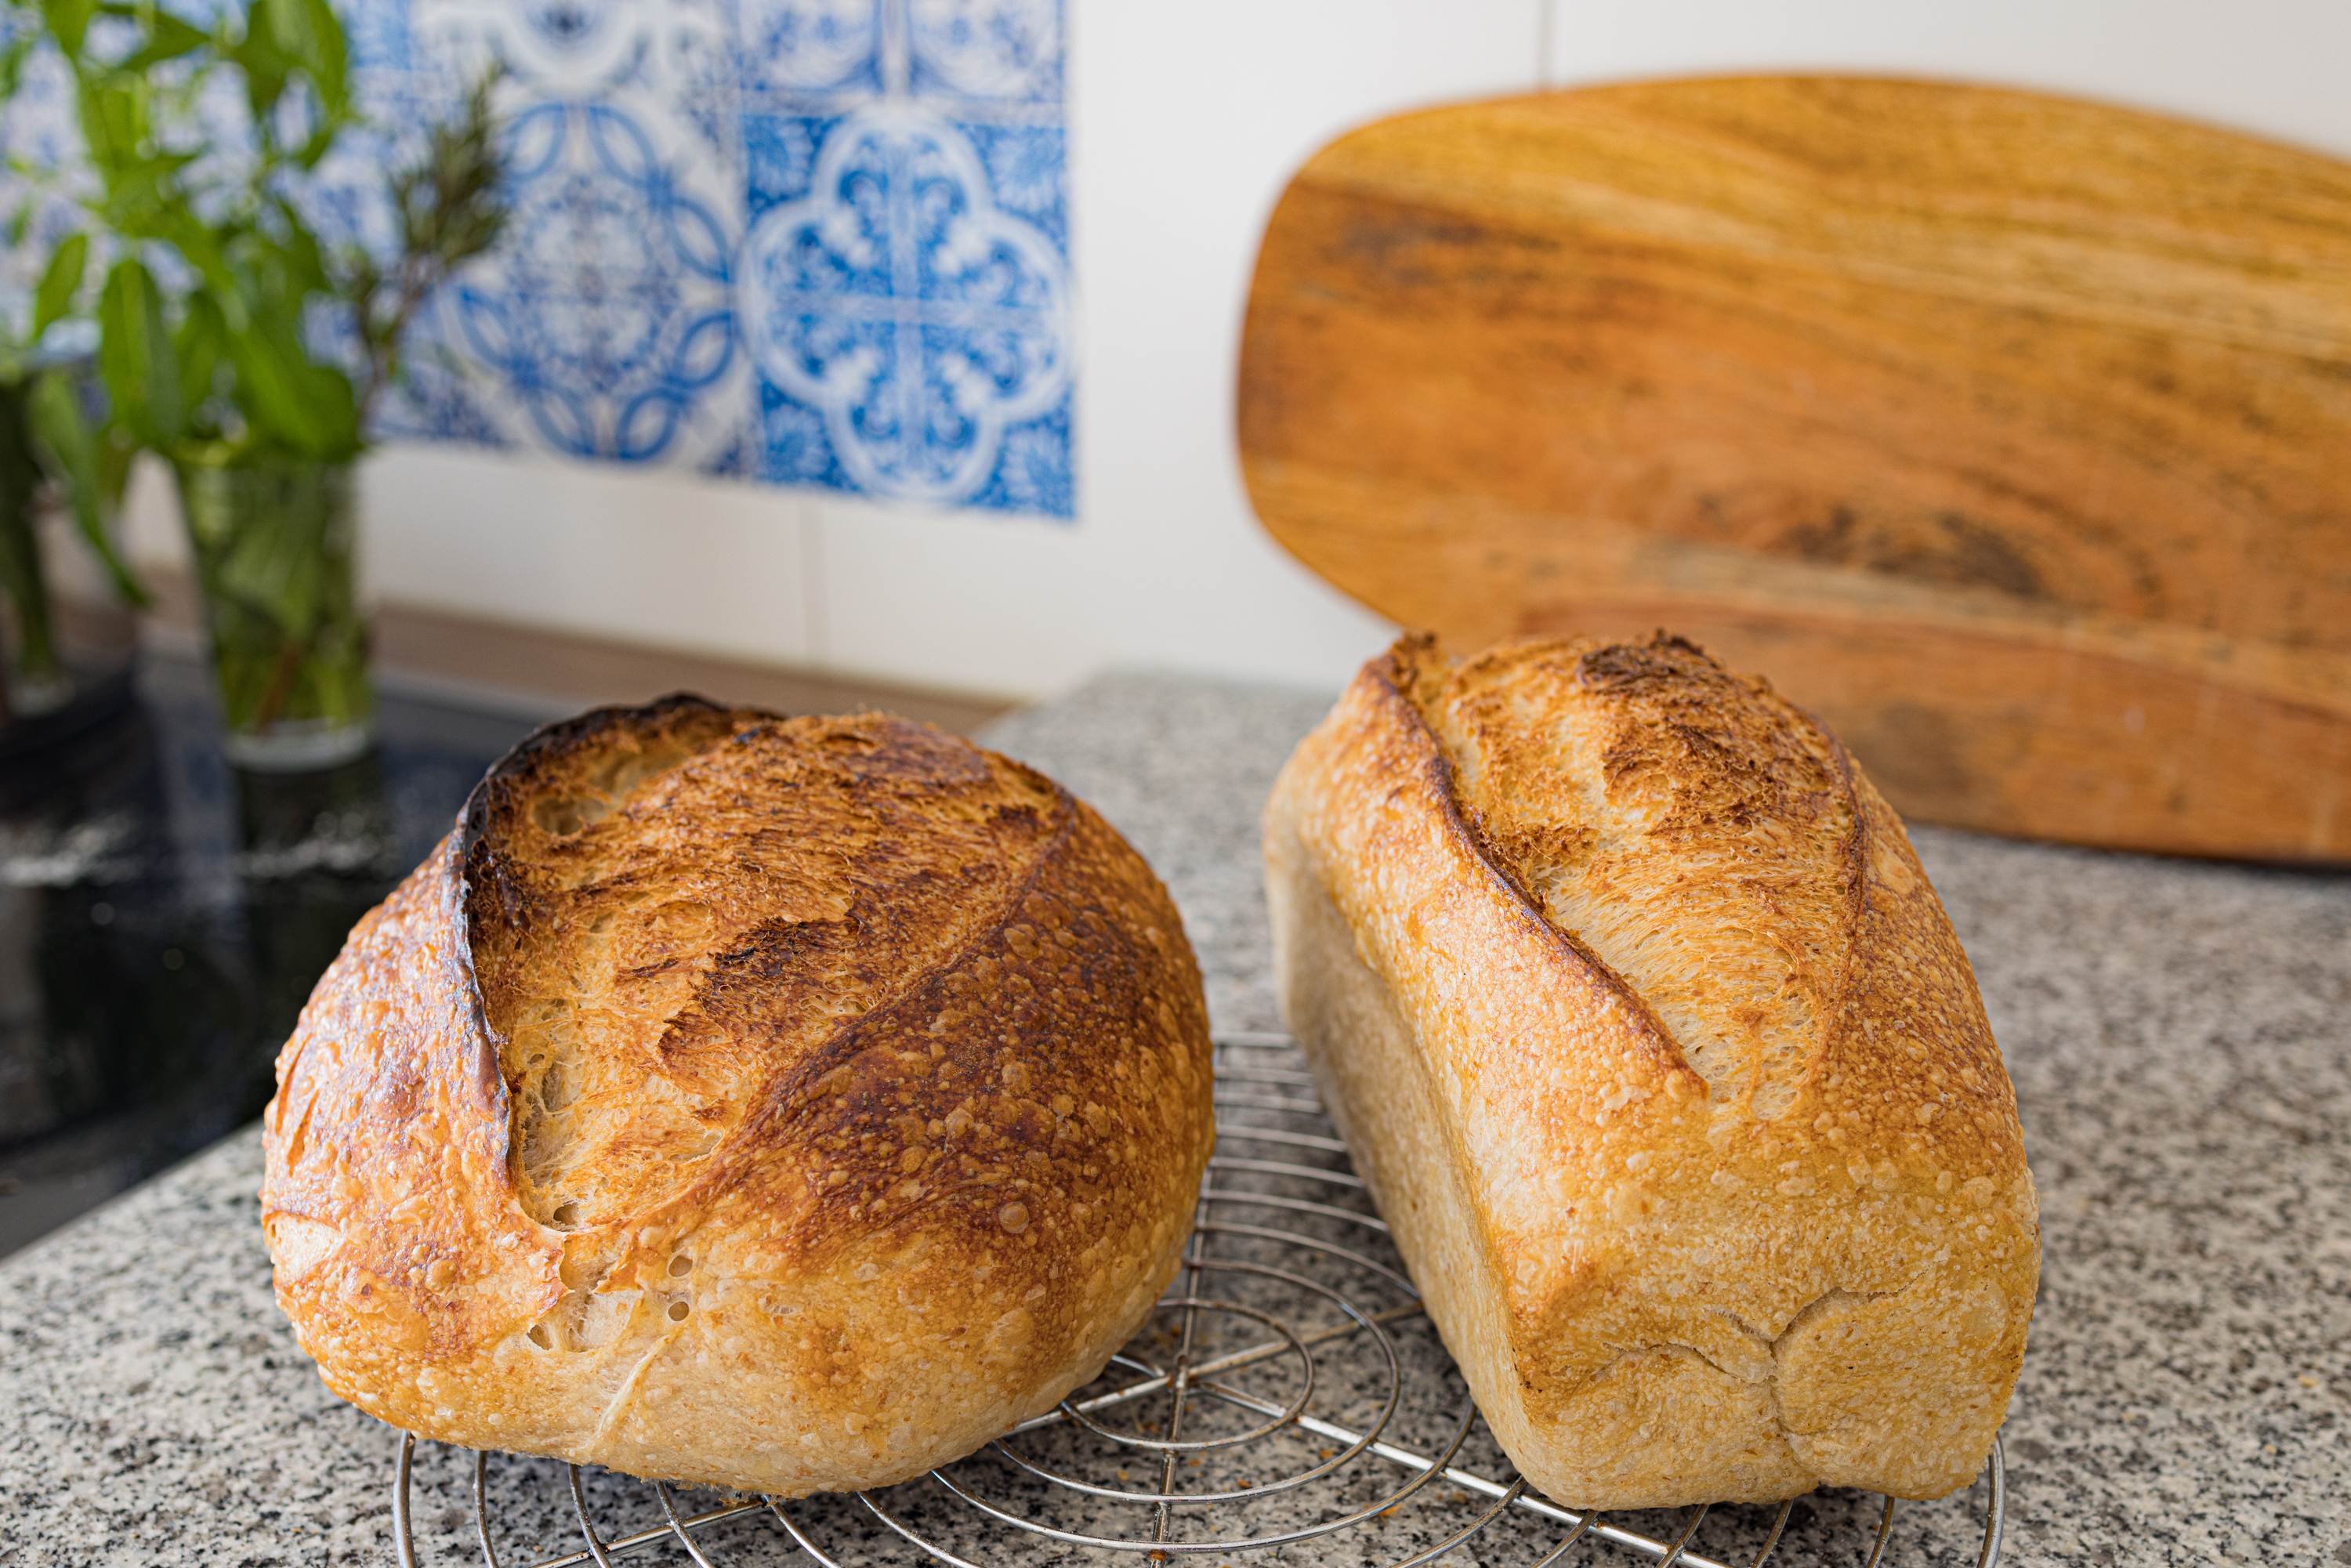
\includegraphics[width=\textwidth]{loaf-pan-free-standing.jpg}
  \caption{A free-standing sourdough bread made with wheat flour}
\end{figure}

A free-standing sourdough bread is my favorite
type of bread. It combines a great crunchy crust, superb
flavor, and a soft fluffy crumb. This is the type of bread
that is being inhaled by my friends and family. Unfortunately
making this type of bread requires a lot more effort, patience,
and technique than other types of bread. You have to perfectly
balance the fermentation process. You can not ferment for too
short and also not for too long. The techniques you need to
learn require a bit more skill. It took me several attempts
to get this right. One of the challenges I faced was that
I had the wrong flour. I didn't properly know how to use my oven.
When should I stop the fermentation? There is a lot of information
out there. I dug through most of it and have tried almost everything.
In many cases the information was wrong, in other cases, I
found another valuable puzzle piece. Aggregating all this
information was one of my main motivations to start the bread code.
My key learning was that there there is no recipe that
you can blindly follow. You will always have to adapt the recipe
to your local available tools and environment.

But do not worry. After reading this chapter you will know
all the signs to look out for. You will be able to read your dough.
You will turn into a confident hobby baker that can bake bread
at home, at high altitudes, at low altitudes, in summer, in winter,
at your friend's place, and even on vacation. Furthermore,
you will know how to scale your production from 1 bread to 100 loaves of bread.
If you ever wanted to open up a bakery, consider this knowledge to
be your foundation.

Mastering this process will enable you to bake amazing bread without
ever buying yeast again.

\section{The process}

\begin{figure}[!htb]
  \includegraphics[width=\textwidth]{sourdough-process-overview.jpg}
  \caption{An overview of the whole sourdough process from start to finish}
\end{figure}

The whole process of making great sourdough bread starts with
readying your sourdough starter. The key to mastering
this process is to manage the fermentation process properly.
For this, the basis is to have an active and healthy
sourdough starter.

Once your starter is ready you proceed to mix all the ingredients.
You want to homogenize your sourdough starter properly. This
way you ensure an even fermentation across your whole dough.

After a short break, you will proceed and create dough strength.
Kneading will create a strong gluten network. This is essential
to properly trap the CO2 created during the fermentation.

Once you kneaded the bulk fermentation starts. Bulk fermentation
because you typically ferment multiple doughs together in one bulk.
Understanding when to stop this step will take some practice.
But nothing to worry about, you will learn the exact signs to look out for.

Once this is completed you need to divide your large blob of
dough into smaller pieces and preshape each piece. This allows
you to apply more dough strength and shape more uniform loaves.

The proofing stage follows where you finish the fermentation process.
Depending on your time you can proof at room temperature or in the fridge.
Mastering proofing will turn your good loaf into a great loaf.

Lastly, you will finish the whole process by baking. You will learn different
options on how to properly steam your dough. This way your
dough will have a beautiful oven spring. During the second
stage of the baking process, you will finish building your crust.

All the steps rely on each other. You will need to get each of
the steps right to make the perfect bread.

\section{Readying your starter}

The most crucial part of the bread-making process is your starter.
The starter is what starts the fermentation in your main dough.
If your starter is off, then your main dough is also going
to cause trouble during the fermentation. Your starter's
properties are passed on to your main dough. If your starter
doesn't have a good balance of yeast to bacteria, so will your
main dough.

\begin{figure}[!p]
  \centering
  \includegraphics[width=\textwidth]{1-ready-starter}
  \caption[Readying a starter]{A flowchart showing how you can prepare your starter before baking.
  This assumes you are using a stiff starter.}
\end{figure}

Generally, think of the dough you are mixing as a big starter with salt.
After mixing all the ingredients you have a green field environment again.
The yeast and bacteria start to fight again to outcompete each other.
There is plenty of food available and they all do their best to win.
Depending on the starter you mix into your dough some of the microorganisms
might have an advantage over the others.

The first option to achieve a good balance is to apply feedings.
If your starter hasn't been fed in a long period the
bacteria dominate. This happens if your starter has been
sitting unused in the fridge for instance. As more and more
acidity piles up the environment is becoming more and more hostile
to the yeast. The lactic acid bacteria tolerate this environment
better. Your dough fermentation would be more towards the
bacterial side with this starter. By applying a couple of
feedings the yeast becomes more active. The older your
starter the more acid resistant the yeast becomes. Initially,
I had to feed my starter 2-3 times to fix the balance. With my
more mature starter, one feeding seems to be enough to balance
the microorganisms.

Some people use a 1:1:1 ratio to refresh the starter. This would
be one part of the old starter (10g for instance), 1 part of flour,
and one part of water. I think this is utter rubbish. As mentioned
your starter is a gigantic dough. You would never a 1:1:1 ratio to
make a dough. You might use a maximum of 20 percent starter to
make a dough. That's why I advocate using a 1:5:5 ratio or a
1:10:10 ratio depending on how ripe your starter is. As I almost
always use a stiffer sourdough starter due to its enhanced
yeast fermentation advantages (see section \ref{section:stiff-starter})
my ratio is never 1:5:5. My ratio would be 1:5:2.5 (1 part old starter,
5 parts flour, 2.5 parts water). If it is very warm where you live
you could opt for the aforementioned 1:10:5 or 1:20:10. This
way you slow down the ripening of your starter. You can use this
trick too to make starter feeding work with your schedule.
If your starter is typically ready in 6 hours but today you need it
ready later, simply increase how much flour/water you feed your starter.
These are all values that you need to experiment with on your own.
Every starter is unique and might behave slightly differently.

The second option at your disposal is the starter quantity that
you use to make the dough. As previously stated your starter
regrows inside of your main dough. While I would normally use
10-20 percent of starter based on the flour, sometimes I go
as low as 1 percent starter. This way the microorganisms have
more room to balance out while fermenting the dough. If my sourdough
starter has not been fed in a day I might use 5 percent of sourdough
to make a dough.  If I push this to 2 days without feedings
I lower the starter amount even further. I would opt for the
previously mentioned 1 percent starter. If the food is very scarce
your microorganisms will sporulate. They need to regrow again
from the spores they created. In this hibernation state, it takes
longer for them to become fully active again. I have tried
several times to make dough directly out of a dry starter.
I wasn't successful because the fermentation took too long.
The microorganisms had to regrow from spores and then begin
the fermentation. As explained earlier there is a limit to
fermentation times as your dough naturally breaks down.
Furthermore, you want your microorganisms to outcompete
other pathogens contained in the flour. The less starter
you use the easier it is for them to reproduce. A strong
starter will outcompete other germs. While the method of
reducing the starter works, I recommend option one more.
It will reliably create better bread. Option 2 is typically
what I use when I fed my starter in the morning but didn't
manage to make a dough in the evening. I don't want to feed
my starter again the next morning. I would like to make a dough
directly without waiting and thus use less of the very ripe starter.

Over time you will become more accustomed to your starter
and how it behaves. You will be able to read the signs of its
activity and judge its state.



\section{Ingredients}
\section{Hydration}
\section{Autolyse}
\section{Fermentolyse}
\section{Dough strength}
\section{Controlling fermentation}
\section{Optional Preshaping}
\section{Shaping}
\section{Proofing}
\section{Scoring}


\chapter{Non wheat bread basics}
\label{chapter:non-wheat-sourdough}
\section{Ingredients}
\section{Managing acidity}
\section{To shape or not to shape}
\section{Proofing}

\chapter{Baking}
Baking refers to the part of the process where you are loading
your dough into the oven. This is typically done after your
dough has gone through the bulk fermentation and proofing stage.

\begin{figure}[!htb]
  \begin{tikzpicture}[node distance = 3cm, auto]
    \node [block] (heat_oven) {\footnotesize Heat oven to 230°C (446°F) for 30 minutes};
    \node [block, right of=heat_oven, node distance=3cm] (score_dough) {\footnotesize Score your dough};
    \node [decision, right of=score_dough, node distance=4cm] (decide_steam) {\footnotesize Choose your steaming method};
    \node [block, below of=heat_oven, node distance=4cm] (inverted_tray_method) {\footnotesize Inverted tray method};
    \node [block, right of=inverted_tray_method, node distance=3cm] (dutch_oven) {\footnotesize Dutch oven};
    \node [block, right of=dutch_oven, node distance=3cm] (steam_injection) {\footnotesize Steam injection oven};
    \node [block, below of=inverted_tray_method, node distance=3cm] (bake_30) {\footnotesize Bake dough for 30 minutes with steam};
    \node [block, right of=bake_30, node distance=3cm] (remove_steam) {\footnotesize Remove source of steam};
    \node [block, right of=remove_steam, node distance=3cm] (build_crust) {\footnotesize Build the crust};
    \node [block, right of=build_crust, node distance=3cm] (finish_baking) {\footnotesize Stop baking 10-30 minutes later depending on crust preference};
    \path [line] (heat_oven) -- (score_dough);
    \path [line] (score_dough) -- (decide_steam);
    \path [line] (decide_steam) -- (inverted_tray_method);
    \path [line] (decide_steam) -- (dutch_oven);
    \path [line] (decide_steam) -- (steam_injection);
    \path [line] (steam_injection) -- (bake_30);
    \path [line] (inverted_tray_method) -- (bake_30);
    \path [line] (dutch_oven) -- (bake_30);
    \path [line] (bake_30) -- (remove_steam);
    \path [line] (remove_steam) -- (build_crust);
    \path [line] (build_crust) -- (finish_baking);
  \end{tikzpicture}
  \caption{A schematic visualization of the baking process using different sources of steam in a home oven.}
  \label{fig:baking-process}
\end{figure}

Some other breads like flat breads
could also be baked on the stove. This chapter is focusing on the
home oven though.

As the dough heats up the water and acids
in your dough start to evaporate. When baking
a gluten based dough the bubbles in your dough start to expand.
Your dough starts to vertically rise. This is called oven spring.
Your bread starts to build a crust of gel like consistency. The crust is still
extensible and can be stretched.

\begin{table}[!htb]
  \centering
  \resizebox{\textwidth}{!}{%
  \begin{tabular}{|l|l|l|}
  \hline
  \textbf{°C  °F} & \textbf{Stage}         & \textbf{Description}                                                                                                                                           \\ \hline
  60 - 140        & Sterilisation          & \begin{tabular}[c]{@{}l@{}}The temperature is too hot for your\\ microorganisms and they die\end{tabular}                                                      \\ \hline
  75 - 167        & Gel building           & \begin{tabular}[c]{@{}l@{}}A gel builds on the surface persisting\\ your dough's structure. It is still\\ extensible and can spring in the\\ oven\end{tabular} \\ \hline
  100 - 212       & Water evaporates       & \begin{tabular}[c]{@{}l@{}}Water begins to evaporate and\\ inflates your dough's alveoli\end{tabular}                                                          \\ \hline
  118 - 244       & Acetic acid evaporates & \begin{tabular}[c]{@{}l@{}}The vinegary tasting acid starts\\ to evaporate. The sourness decreases\end{tabular}                                                \\ \hline
  122 - 252       & Lactic acid evaporates & \begin{tabular}[c]{@{}l@{}}The dairy tasting lactic acid begins\\ to evaporate. Sourness further decreases\end{tabular}                                        \\ \hline
  140 - 284       & Maillard reaction      & \begin{tabular}[c]{@{}l@{}}The maillard reaction starts to deform\\ starches and proteins. The dough starts\\ browning\end{tabular}                            \\ \hline
  170 - 338       & Caramelization         & \begin{tabular}[c]{@{}l@{}}Remaining sugars begin to caramelise\\ giving your bread a distinct flavor\end{tabular}                                             \\ \hline
  \end{tabular}%
  }
  \caption{The different stages of the baking process and their impact on your bread}
\end{table}

At around 60°C (140°F) the microbes in your dough start to die.
There are rumors that until this happens the microbes produce
a lot of CO2, resulting in the dough's expansion. This temperature
is however reached quickly. Furthermore stress makes the microbes
enter sporulation mode in order to focus on spreading genetics.
More research should be done here to validate or invalidate this
claim.

At 75°C (167°F) the surface of your dough turns into a gel. It
holds together nicely and is still extensible. This gel is essential
for oven spring as it retains the gas of your dough very well.

At around 100°C (212°F) the water starts to evaporate out of your
dough. If this wasn't the case your dough would taste soggy and
doughy. The higher hydration your dough has the more water your bread
still contains after the bake. The crumb is going to taste a bit
more moist. The consistency will be different.

Another often undervalued step is the evaporation of acids. At
118°C (244°F) the acetic acid in your dough starters to evaporate.
Shortly after at 122°C (252°F) the lactic acid begins evaporating.
This is crucial to understand and opens a door to many interesting
ways to influence your final bread's taste. As more and more water
begins to evaporate the acids in your dough become more concentrated.
There is less water but in relation you have more acids. So a shorter
bake will lead to a more tangy dough. The longer you bake the bread
the more of the water evaporates, but also ultimately the acids will follow.
They will be more concentrated. In absolute units though they
will become less and less. The longer you bake the less sour
your bread is going to be. So by baking you can
influence which sourness level you would like to achieve.

\begin{figure}[!htb]
  \includegraphics[width=\textwidth]{baking-experiment-temperatures.png}
  \caption{This chart shows how surface temperatures change using
  different steaming methods. In this case I used a dutch oven and an apple as
  dough replacement. All the apples were coming from the fridge. The temperature
  was measured using a barbecue thermometer.
  The more steam the faster the surface temperature increases.}
\end{figure}

It would be a very interesting experiment to bake a bread at different exact
temperatures. How would a bread taste with only evaporated water but
full acidity? What if you were to just completely get rid of the acetic
acid? How would the taste change?

As the temperature increases
the crust thickens. The maillard reaction kicks in further deforming
proteins and starches. The outside of your dough starts to become
browner and crisper. This process begins at around 140°C (284°F)

Once the temperature increases even more to around 170°C (338°F)
the caramelization process begins. The remaining sugars the microbes
did not convert yet start to brown and darken. You can keep baking
for as long as you like to achieve the crust color that you like.
\footnote{This really depends a lot on your personal preference.
Some people prefer a darker crust, others prefer a more pale crust.
It's better to build less crust than too much. You can always just
heat your bread in the oven one more time to continue building a
darker crust.}

The best option to know that your dough is done is to take
the temperature of your dough. You can use a barbecue thermometer
to measure it. Once the core temperature is at around 92°C (197°F)
you can stop the baking process. This is typically not done though
as the crust hasn't been built yet.\footnote{The thermometer is
especially important when using a large loaf pan. It is sometimes
very hard to judge from the outside if the dough is done. I failed
many times and ended up having a semi baked dough.}

Once your dough has finished baking it is ready to eat. Your
dough has turned into a bread. At this
point your bread is sterile as the temperature was too hot for
for the microorganisms to survive.

\section{The role of steam}

Steam is essential when baking as it helps to counter premature
crust building. During the first stage of the bake the dough
increases in size. The water in your dough evaporates and pushes
the whole dough upwards. 

\begin{figure}[!htb]
  \includegraphics[width=\textwidth]{baking-process-steam.jpg}
  \caption{How steam builds in your oven using the later described
  inverted tray method}
\end{figure}

Normally under high heat a crust would form. Just like
if you were to bake vegetables in your home oven. At some point
they become darker and crisper. This is the same thing that
happens with your dough. You want to delay this process
as long as possible until your dough no longer expands.
Expansion stops when most of the microbes have died and
the evaporating water no longer stays inside the alveoli.
The stronger the gluten network the more gas can be retained
during the baking process. This gluten network at some point
loses its ability to contain gas as the temperature heats
up. The dough stops increasing in size. The steam plays
an important role as it condenses and evaporates on top
of your dough. The surface temperature is rapidly increasing
to around 75°C (160°F). At this temperature the gel starts
to build. This gel is still extensible and allows expansion.
Without the steam the dough would never enter the gel stage,
but instead directly go to the maillard reaction zone. You
want your dough to stay in this gel stage as long as possible
to achieve maximum expansion.\footnote{You can remove your
dough from the oven after 5 minutes to see the gel. You will notice
that it holds the dough's structure. It has a very interesting consistency.}

\begin{figure}[!htb]
  \includegraphics[width=\textwidth]{baking-process-stage-2.jpg}
  \caption{The second stage of the bake is done without steam to build
  a thicker darker crust}
\end{figure}

When not steaming enough you will notice that the scoring
incisions do not properly open up during the bake. They stay
closed as the dough is unable to push through the crust.

Another common sign is that you have larger pockets
of air towards the crust of your dough. As the dough increases
vertically, expansion is halted by the crust. The pockets
of air converge into larger pockets as the pressure increases.
This can also happen when you are baking at too high a temperature.

The more you steam, the softer your dough's crust is. You will never
enter the maillard and caramelization stage. This
is the reason why the source of steam is removed
for the second stage of the bake. No more expansion can
happen and you can focus on building a crust. If you
would like a soft crust you can steam your dough all the
way.

\begin{figure}[!htb]
  \includegraphics[width=\textwidth]{baking-too-hot.jpeg}
  \caption{A submission by Karomizu showing a bread that has been baked
  at too high a temperature or with too little steam. Note the large
  pockets of air towards the crust. They are a typical indicator.}
\end{figure}

\section{Dutch ovens}

Dutch ovens are an ideal way to bake with a lot of
steam. They are not fully sealed. Regardless though,
as water evaporates from your dough it will create a steamy
environment allowing your dough to rise. It really
makes baking in a home oven very easy.

When using a dutch oven make sure to preheat it properly,
this way your dough will not stick to it. You can also
use additional semolina flour or parchment paper. Another
good trick is to spritz your dough with a bit of water.
To create more steam you could also place a small ice cube
next to your main dough.

I have been using a dutch oven myself for a long time. They
have issues though. They are relatively heavy. It is dangerous
to operate hot cast iron ovens. Especially when working with steam
you have to be very careful.  Furthermore
they are expensive to buy. If your dutch oven is made out
of cast iron you have to season it from time to time. This takes
time.

The biggest disadvantage though is
capacity. You can only bake a single bread at the
same time. In many cases it makes sense to bake multiple
loaves in one go. It makes the whole process more
efficient as you have to knead less per loaf. The time it
takes to make one bread significantly reduces. Furthermore
you don't require as much energy. You don't have
to preheat your oven twice for each individual loaf.


\section{Inverted tray method}

The inverted tray method simulates a dutch oven.
By placing another tray on top of your dough the steam
created from the dough and water source stays
around your dough.

\begin{figure}[!htb]
  \begin{tikzpicture}[node distance = 3cm, auto]
    \node [block] (init) {\footnotesize Place water tray and stone in oven};
    \node [block, right of=init] (heat_oven) {\footnotesize Heat oven to 230°C (446°F) for 30 minutes};
    \node [block, right of=heat_oven] (score_your_dough) {\footnotesize Score your dough};
    \node [block, right of=score_your_dough] (spritz) {\footnotesize Spritz your dough with water};
    \node [block, right of=spritz] (load_tray) {\footnotesize Place non-preheated inverted tray in oven};
    \node [block, below of=load_tray, node distance=4cm] (load_doughs) {\footnotesize Load doughs into oven};
    \node [block, left of=load_doughs, node distance=3cm] (load_water) {\footnotesize Place water in heated water tray};
    \node [block, left of=load_water, node distance=3cm] (bake) {\footnotesize Bake 30 minutes or until core temperature is 92°C (197°F)};
    \node [block, left of=bake, node distance=3cm] (remove_steam) {\footnotesize Remove steam source and top tray};
    \node [block, left of=remove_steam, node distance=3cm] (finish) {\footnotesize Bake at least another 10 minutes or until crust has your desired color};
    \path [line] (init) -- (heat_oven);
    \path [line] (heat_oven) -- (score_your_dough);
    \path [line] (score_your_dough) -- (spritz);
    \path [line] (spritz) -- (load_tray);
    \path [line] (load_tray) -- (load_doughs);
    \path [line] (load_doughs) -- (load_water);
    \path [line] (load_water) -- (bake);
    \path [line] (bake) -- (remove_steam);
    \path [line] (remove_steam) -- (finish);
  \end{tikzpicture}
  \caption{A schematic visualization the inverted tray baking method that works great for home ovens.}
  \label{fig:inverted-tray-process}
\end{figure}


The biggest advantage of this method compared to the
dutch oven is scalability. You can bake multiple loaves
at the same time. In my case that is around 2 freestanding
loaves and 4 loaves in a loaf pan.

For the inverted tray you will need the following tools:
\begin{itemize}
\item 2 trays
\item 1 heat resistant bowl
\item Boiling water
\item Oven gloves
\item Optional parchment paper
\end{itemize}

\begin{figure}[!htb]
  \includegraphics[width=\textwidth]{baking-example.jpg}
  \caption{My home oven setup}
\end{figure}

These are the steps to follow with the inverted tray method:
\begin{enumerate}
\item Preheat the oven to around 230°C (446°F) and 
preheat one of the trays.
\item Bring water to boil.
\item Place your doughs on a piece of parchment paper. You
can also place each on a tiny piece of parchment paper.
this makes loading the dough easier. If you don't
have it or don't want to use it, you can opt for 
semolina flour. It helps to make the tray non stick.
\item Take out your hot tray and place it
on a cooling rack, or on something else that
is heat resistant.
\item Score your doughs.
\item Place your doughs on the hot tray.
\item Place the cold tray in your oven in an inverted position.
\item Move your hot tray including the loaves back
to the oven.
\item Place the boiling water in the heat resistant
water bowl. I have added rocks to it, it helps
to improve the steam even further. This is optional.
\item Close the oven.
\item After 30 minutes remove the top tray. Also remove the bowl with water.
\item Finish baking your bread until you have reached your desired
crust color. In my case this is another 15-25 minutes typically.
\end{enumerate}

\section{Conclusions}

\begin{table}[]
  \centering
  \resizebox{\textwidth}{!}{%
  \begin{tabular}{|l|l|l|l|}
  \hline
  \textbf{Oven type}                                                         & \textbf{Plain (no tools)} & \textbf{Inverted tray} & \textbf{Dutch oven} \\ \hline
  Gas                                                                        & No                        & No                     & Yes                 \\ \hline
  \begin{tabular}[c]{@{}l@{}}Convection\\ (Fan always on)\end{tabular}       & No                        & No                     & Yes                 \\ \hline
  \begin{tabular}[c]{@{}l@{}}Convection\\ (Fan can be disabled)\end{tabular} & No                        & Yes                    & Yes                 \\ \hline
  Steam                                                                      & Yes                       & Yes                    & Yes                 \\ \hline
  \end{tabular}%
  }
  \caption{An overview of ovens and their different baking methods}
\end{table}

Depending on your home oven a different method
of steaming should be used. Generally most ovens
are made to vent out most of the steam during the
bake. They are typically not fully closed. During
baking you want to dry out whatever you are baking.
This is ideal if you are baking vegetables and
want them to dry out. For baking though this is
highly problematic. As described earlier, you
want there to be as much steam as possible.

If you are using a gas based oven, the only option
is to utilize a dutch oven. The same is true when you
are using a convection oven with a fan that
cannot be disabled. When using a convection
oven with a fan that can be turned off, you can
opt to use the cost efficient inverted tray
method.

If you are in the luxurious
position of owning a steam oven, things are easier.
Just activate the steam function and you are
good to go. Placing an additional tray on top of your
dough during the bake helps to bake with indirect
heat. You remain in the gel zone longer and
will experience more oven spring.


\chapter{Storing bread}
\section{Fridge}
\section{Room temperature}
\section{Frozen}

\chapter{Troubleshooting}

\section{Debugging your crumb structure}%
\label{section:debugging-crumb-structure}

The crumb structure of your bread provides insights into how well
your fermentation process has gone. You can also spot common flaws
arising from improper technique. This chapter will provide you with information
that you can use to debug your baking process.

\begin{figure}
  \includegraphics[width=\textwidth]{crumb-structures-book}
  \caption[Debugging your crumb structure]{A schematic visualization of
      different crumb structures and their respective causes. The final bread's
      crumb is a key aspect to identify potential issues related to
      fermentation or baking technique.}%
  \label{fig:crumb-structures-book}
\end{figure}

\subsection{Perfect fermentation}

\begin{figure}
  \includegraphics[width=\textwidth]{open-crumb}
  \caption[Perfectly fermented bread]{The bread has a somewhat open crumb
      with areas featuring a honeycomb structure.}%
  \label{fig:open-crumb}
\end{figure}

Of course the perfect fermentation is debatable and highly subjective. To
me the perfect sourdough bread features a crisp crust paired with a fluffy,
somewhat open crumb. This is the perfect balance of different consistencies
when you take a bite.

Some people are chasers of a very open crumb, meaning you have large pockets
of air (alveoli). It's subjective whether that's the style of bread that you like;
however, to achieve it you need to ferment your bread dough perfectly.
It takes a lot of skill both in terms of mastering fermentation and technique
to achieve a crumb structure like that.

Personally, I~like a bread like that, just with a slightly less wild crumb.
The style of crumb I~like is called the \emph{honeycomb crumb}. It's not too open, but
just enough open to make the bread very fluffy. To achieve the previously mentioned open crumb, you
have to touch your dough as little as possible. The more you interact with your
dough, the more you are degassing your dough. Excess touching of the dough
results in the dough's alveoli merging together. The crumb will not be as open.
That's why achieving such a crumb works best if you only ferment
one loaf at a time. Normally, if you have to pre-shape your dough,
you will automatically degas your dough a little bit during the rounding process.
If you skip this step and directly shape your dough, you will achieve a more open crumb.
A good rule of thumb is to not touch your dough for at least 1--2~hours before shaping,
to achieve as open a crumb as possible.

\begin{figure}
  \includegraphics[width=\textwidth]{honeycomb}
  \caption[Honeycomb crumb structure]{A whole-wheat sourdough with an almost
      exclusive honeycomb crumb structure.}%
  \label{fig:honeycomb}
\end{figure}


Now this is problematic when you want to
make multiple loaves at the same time. Pre-shaping is essential as you are required
to divide your large bulk dough into smaller chunks. Without the pre-shaping
process, you would end up with many non-uniform bread doughs. This technique is
also used when making ciabattas. They are typically not shaped. You only cut the
bulk dough into smaller pieces, trying to work the dough as little as possible.
With pre-shaping you will converge your dough's alveoli into more of a honeycomb structure,
as large pockets of air will slightly merge. Similarly to the open crumb structure,
you also have to nail the fermentation process perfectly to achieve this crumb.
Too long a fermentation will result in gas leaking out of your dough while baking.
The honeycombs won't be able to retain the gas. If you ferment for too short a time,
there is not enough gas to inflate the structures. To me this is the perfect
style of crumb. As someone who appreciates jam, no jam will fall through a slice
of this bread compared to an open crumb.

\subsection{Overfermented}%
\label{subsec:overfermented-dough}

\begin{figure}
  \includegraphics[width=\textwidth]{fermented-too-long}
  \caption[Overfermented sourdough bread]{A relatively flat dough that has many tiny pockets of air.}%
  \label{fig:fermented-too-long}
\end{figure}

When fermenting your dough for too long, the protease enzyme starts to
break down the gluten of your flour. Furthermore, the bacteria consume the gluten
in a process called \emph{proteolysis}~\cite{raffaella+di+cagno}.
Bakers also refer to this process as \emph{gluten rot}.
The gluten that normally traps the \ch{CO2} created
by the fermentation process of your microorganisms can no longer keep the
gas inside of the dough. The gas disperses outward resulting in smaller alveoli in your crumb.
The bread itself tends to be very flat in the oven. Bakers often refer
to this style of bread as a \emph{pancake}. The oven spring can be compared
to bread doughs made out of low-gluten flour like einkorn.

Your bread will feature a lot of acidity, a really strong distinctive tang. From
a taste perspective, it might be a little bit too sour. From my own tests with family and
friends (n=15--20), I~can say that this style of bread is typically
appreciated less. However, I~personally really like the hearty strong taste.
It is excellent in combination with something
sweet or a soup.  From a consistency perspective, it is no longer as fluffy as it could be.
The crumb might also taste a little bit gummy. That's because it has been broken down a lot
by the bacteria. Furthermore, this style of bread has a significantly lower amount
of gluten~\cite{raffaella+di+cagno} and is no longer comparable to raw flour,
it's a fully fermented product.
You can compare it with a blue cheese that is almost lactose free.

When trying to work with the dough, you will notice that suddenly the dough feels
very sticky. You can no longer properly shape and work the dough. When trying to
remove the dough from a banneton, the dough flattens out a lot. Furthermore,
in many cases your dough might stick to the banneton. When beginning with baking
I~would use a lot of rice flour in my banneton to dry out the surface of the dough a lot.
This way the dough wouldn't stick, despite being overfermented. However as it
turns out the stickiness issue has been my lack of understanding the fermentation
process. Now I~never use rice flour, except when trying to apply decorative scorings.
Managing properly fermentation results in a dough that is not sticky.

If you are noticing, during a stretch and fold or during shaping, that your dough
is suddenly overly sticky, then the best option is to use a loaf pan. Simply take
your dough and toss it into a loaf pan. Wait until the dough mixture has increased
in size a bit again and then bake it. You will have a very good-tasting sourdough
bread. If it's a bit too sour, you can just bake your dough for a longer period
of time to boil away some of the acidity during the baking process. You can also use
your dough to set up a new starter and try again tomorrow. Lastly, if you are hungry,
you can simply pour some of your dough directly into a heated pan with a bit of
oil. It will make delicious sourdough flatbreads.

To fix issues related to over-fermentation, you need to stop the fermentation process
earlier. What I~like to do is to extract a small fermentation sample from my dough.
Depending on the volume increase of this sample, I~can mostly judge when my fermentation
is finished. Try to start with a \qty{25}{\percent} volume increase of your
main dough or sample.  Depending on how much gluten your flour has, you can
ferment for a longer period of time.  With a strong flour featuring a
\qtyrange{14}{15}{\percent} protein, you should be able to safely ferment
until a \qty{100}{\percent} size increase. This however also depends on your
sourdough starter's composition of yeast and bacteria. The more bacterial fermentation,
the faster your dough structure breaks down. Frequent feedings of your sourdough
starter will improve the yeast activity. Furthermore, a stiff sourdough starter
might be a good solution too. The enhanced yeast activity will result in a more fluffy
dough with less bacterial activity. A better yeast activity also will result
in less acidity in your final bread. If you are a chaser of a very strong tangy
flavor profile, then a stronger flour with more gluten will help.

When retarding sourdough (cold-proofing in the refrigerator), temperature plays a
pivotal role in fermentation rates.  As the dough chills in the refrigerator,
fermentation decelerates. Starting the retarding process at a warmer
temperature means this deceleration takes longer.

For instance, a dough that's ideal after 8 hours of retarding might be ready in
merely 4~hours if it began at a higher temperature. Thus, it's crucial to
experiment and determine the optimal retarding duration for your specific
conditions. Conversely, if the dough starts colder, fermentation halts more
rapidly in the refrigerator. In such scenarios, allowing the dough to proof at
room temperature briefly before refrigerating can be beneficial.

\subsection{Underfermented}

\begin{figure}
  \includegraphics[width=\textwidth]{fermented-too-short-underbaked}
  \caption[Underfermented bread]{A dense dough featuring a gummy, not fully
      gelatinized area.  The picture has been provided by the user wahlfeld
      from our community Discord server.}%
  \label{fig:fermented-too-short-underbaked}
\end{figure}

This defect is also commonly referred to as \emph{underproofed}. However underproofed
is not a good term as it only refers to having a short final
proofing stage of the bread-making process.
If you were to bake your bread after a perfectly-timed bulk fermentation stage,
the result will not be underproofed even if you skipped the proofing stage entirely.
Proofing will make your dough a bit more extensible and allows your sourdough
to inflate the dough a bit more. When faced with an underfermented bread, something
went wrong earlier during the bulk fermentation stage, or maybe even
before with your sourdough starter.

A typical underfermented dough has very large pockets of air and is partially
wet and gummy in some areas of the dough. The large pockets can be compared
to making a non-leavened wheat or corn tortilla. As you bake the dough in your pan,
the water slowly starts to evaporate. The gas is trapped in the structure of the dough
and will create pockets. In case of a tortilla, this is the desired behavior.
But when you observe this process in a larger dough, you will create several
super alveoli. The water evaporates, and the first alveoli form. Then at some point,
the starch starts to gelatinize and becomes solid. This happens first inside of the pockets
as the interior heats up faster compared to the rest of the dough. Once all the starch
has gelatinized, the alveoli holds their shape and no longer expand. During this
process other parts of the bread dough are pushed outwards. That's why an underfermented
dough sometimes even features an ear during the baking process. This
is also commonly referred to as a \emph{fool's crumb}. You are excited about an ear which
can be quite hard to achieve. Plus you might think you finally created some big pockets
of air in your crumb. But in reality you fermented for too short a period
of time.

\begin{figure}
  \includegraphics[width=\textwidth]{fools-crumb}
  \caption[Fool's crumb large alveoli]{A typical example of a fool's crumb
      featuring an ear and several overly large alveoli. The picture has been
      provided by Rochelle from our community Discord server.}%
  \label{fools-crumb}
\end{figure}

In a properly fermented dough, the alveoli help with the heat transfer throughout the dough.
From within the many tiny fermentation-induced pockets, the starch gelatinizes. With
an underfermented dough, this heat transfer does not properly work. Because of that
you sometimes have areas which look like raw dough. Bakers refer to this as a very
gummy structure sometimes. Baking your dough for a longer period of time would also properly
gelatinize the starch in these areas. However, then other parts of your bread
might be baked too long.

To fix issues related to under-fermentation, you simply have to ferment your dough
for a longer period of time. Now, there is an upper limit to fermentation time
as your flour starts to break down the moment it is in contact with water. That's why it
might be a good idea to simply speed up your fermentation process. As a rough
figure, I~try to aim for a bulk fermentation time of around 8--12~hours typically.
To achieve that you can try to make your sourdough starter more active.  This can be done
by feeding your starter daily over several days. Use the same ratio as you would
do for your main bread dough. Assuming you use \qty{20}{\percent} starter
calculated on the flour, use a 1:5:5 ratio to feed your starter. That would be
\qty{10}{\gram} of existing starter, \qty{50}{\gram} of flour, \qty{50}{\gram}
of water for instance.  To boost your yeast activity even more, you can
consider making a stiff sourdough 
starter. The bacteria produces mostly acid. The more acidity
is piled up, the less active your yeast is. The stiff sourdough starter
enables you to start your dough's fermentation with stronger yeast activity
and less bacterial activity.

\subsection{Not enough dough strength}

\begin{figure}
  \includegraphics[width=\textwidth]{flat-bread}
  \caption{A very flat bread without enough dough strength.}%
  \label{flat-bread}
\end{figure}

When a dough flattens out quite a lot during the baking process, the chances are
that you did not create enough dough strength. This means your gluten matrix
hasn't been developed properly. Your dough is too extensible and flattens out
mostly rather than springing upwards in the oven. This can also happen if you
proofed your dough for too long. Over time the gluten relaxes and your dough
becomes more and more extensible. You can observe the gluten relaxing behavior
too when making a pizza pie. Directly after shaping your dough balls, it's
very hard to shape the pizza pie. If you wait for 30--90~minutes stretching
the dough becomes a lot easier.

The easiest way to fix this is probably to knead your dough more at the start. To simplify
things consider using less water for your flour too. This will result in a more elastic dough
right away. This concept is commonly used for no-knead style sourdough.  Alternatively, you
can also perform more stretch and folds during the bulk fermentation process. Each
stretch and fold will help to strengthen the gluten matrix and make a more elastic dough.
The last option to fix a dough with too little dough strength is to shape your dough tighter.

\subsection{Baked too hot}

\begin{figure}
  \includegraphics[width=\textwidth]{baked-too-hot-v2}
  \caption{A bread with very large alveoli close to the crust.}%
  \label{baked-too-hot}
\end{figure}

This is a common mistake that has happened to me a lot. When you bake your dough
at too high a temperature, you constrain your dough's expansion. The starch
gelatinizes and becomes more and more solid. At around
\qty{140}{\degreeCelsius} (\qty{284}{\degF}) the Maillard reaction starts to
completely thicken your bread dough's crust. This is similar to baking your
bread dough without steam. As the internal dough's temperature heats up,
more and more water evaporates, gas expands and the dough is being pushed upwards.
Once the dough reaches the crust, it can no longer expand. The alveoli merge
into larger structures close to the surface of the dough. By baking too hot,
you are not achieving the ear which adds extra flavor. Furthermore, by restricting
it's expansion, the crumb will not be as fluffy as it could be.

If you have an extensible dough with high hydration, baking too cold will result
in the dough flattening out quite a lot. The gelatinization of the starch is
essential for the dough to hold its structure. After conducting several
experiments, it seems that my sweet spot for maximum oven spring seems to be
at around \qty{230}{\degreeCelsius} (\qty{446}{\degF}). Test the temperature
of your oven, because in several
cases the displayed temperature might not match the actual temperature of your
oven~\cite{too+hot+baking}. Make sure to turn off the fan of your oven. Most
home ovens are designed to vent the steam as fast as possible. If you can not
turn the fan off, consider using a Dutch oven.

\subsection{Baked with too little steam}

\begin{figure}[h]
  \includegraphics[width=\textwidth]{no-steam}
  \caption[Bread baked with too little steam]{One of my earlier breads that
      I~baked at a friend's place where I~couldn't steam the dough properly.}%
  \label{no-steam}
\end{figure}

Similar to baking too hot, when baking without enough steam, your dough's crust
forms too quickly. It's hard to spot the difference between the two mistakes.
I~typically first ask about the temperature and then about the steaming technique
to determine what might be wrong with the baking process. Too little steam can
typically be spotted by having a thick crust around all around your dough paired
with large alveoli towards the edges.

The steam essentially prevents the Maillard reaction from happening too quickly
on your crust. That's why steaming during the first stages of the bake is so important.
The steam keeps the temperature of your crust close to around
\qty{100}{\degreeCelsius} (\qty{212}{\degF}). Achieving steam
can be done by using a Dutch oven, an inverted tray and/or a bowl of boiling water.
You might also have an oven with a built-in steam functionality. All the methods work,
it depends on what you have at hand. My default go-to method is an inverted
tray on top of my dough, paired with a bowl full of boiling water towards the bottom
of the oven.

\begin{figure}[ht]
  \includegraphics[width=\textwidth]{apple-experiment-temperatures}
  \caption[Measuring ambient and surface temperature]{An apple with 2 probes
      to measure ambient and surface temperatures of several steaming
      techniques in a Dutch oven.}%
  \label{apple-experiment-temperatures}
\end{figure}

Now there can also be too much steam. For this I~tested using a Dutch oven paired with large ice
cubes to provide additional steam. The temperature of my dough's surface would directly
jump close to 100°C. The steam contains more energy and thus through convection
can heat up the surface of your dough faster. I~tested this by putting an apple inside
a Dutch oven and measuring its surface temperature using a barbecue thermometer.
I~then changed the steaming methods to plot how quickly the temperature
close to the surface changes. I~tested an ice cube inside of a preheated
Dutch oven, a plain preheated Dutch oven, a preheated Dutch oven with spritzes
of water on the apple's surface and a non-preheated Dutch oven where I~would only preheat
the bottom part. The experiment then showed that the ice-cube method would heat up
the surface of the apple a lot quicker. When replicating this with a bread dough,
I~would achieve less oven spring.

\begin{figure}[ht]
  \includegraphics[width=\textwidth]{apple-experiment-surface-temperatures}
  \caption[Surface temperature versus steaming technique]{A chart showing how
      the temperature of the apple's surface changes with different
      steaming techniques.}%
  \label{apple-experiment-surface-temperatures}
\end{figure}

\begin{figure}[ht]
  \includegraphics[width=\textwidth]{apple-experiment-ambient-temperatures}
  \caption[Dutch Oven temperature versus steaming technique]{This figure shows
      how the ambient temperatures inside of the Dutch oven change depending
      on the steaming technique that is used.}%
  \label{apple-experiment-ambient-temperatures}
\end{figure}

Generally though, achieving too much steam is relatively challenging. I~could only
make this mistake when using a Dutch oven as the steaming method paired with relatively
large ice cubes. After talking with other bakers using the same Dutch oven, it seems
that my ice cubes (around \qty{80}{\gram}) were 4 times as heavy as the ones
other bakers would use (\qty{20}{\gram}).

\section{Baking in the tropics}

Depending on the temperature your fermentation speed adapts.
In a warmer environment everything is faster. In a colder
environment everything is slower.

This includes the speed at which your sourdough ferments
the dough but also the speed of enzymatic reactions. The
amylase and protease enzymes work faster, making more
sugars available and degrading the gluten proteins.

At around 22°C in my kitchen my bulk fermentation is ready
after around 10 hours. I am using around 20 percent of sourdough
starter based on the flour. In summer times the temperatures
in my kitchen sometimes increase to 25°C. In that case
I am reducing the sourdough starter to around 10 percent.
If I wouldn't do that my fermentation would be done after
around 4-7 hours. The problem is that the dough is quite
unstable when fermenting at this high speed. This means
that you are easily running into issues of overfermentation.
Finding the perfect sweet spot between fermenting enough
and not too much is becoming much harder. Normally you might
have a time window of 1 hour. But at the rapid speed it
might be reduced to a time window of 20 minutes. Now at
30°C ambient temperature things are way faster. Your bulk
fermentation might be complete in 2-4 hours when using
10-20 percent starter. Proofing your dough in the fridge
becomes almost impossible. As your dough cools down in the
fridge the fermentation also slows down. However cooling the
dough down from 30°C to 4-6°C in your fridge takes much
longer. Your dough is much more active compared to a dough
that starts at a temperature of 20-25°C. You might
end up overproofing your dough if you leave it overnight
in the fridge.

That's why I recommend that you reduce the amount of starter
that you use in the tropics to something at around 1-5 percent
based on the flour. This will slow down the fermentation
process significantly and provides you a bigger window
of time. Try to aim for an overall bulk fermentation of at
least 8-10 hours. Reduce the amount of starter to get there.

When making a dough try to use the same water temperature
as your ambient temperature. Assuming that the temperature
will climb to 30°C, try to start your dough directly
with 30°C water. This means that you can carefully rely on
a small fermentation probe that visualizes your fermentation
progress. The probe only works reliably if your dough temperature
is equal to your ambient temperature. Else the sample heats
up or cools down faster. So tread carefully when using
the sample in this case. It's always better to stop
the fermentation a little too early rather than too late.
Stretch and folds during the bulk fermentation
will help you to develop a better look and feel for
the dough. An expensive but possibly useful tool
could be a pH meter that allows you to perfectly
measure how much acidity has been created by the
lactic and acetic acid bacteria. In this case measure
the pH repeatedly and figure out a value that works
for your sourdough. In my case I tend to end bulk
fermentation at a pH of around 4.1. Please don't just
follow my pH value, it's very individual. Keep measuring
with different doughs to find out a value that works for you.

\section{My bread stays flat}
\section{I want more tang in my bread}
\section{My bread is too sour}
\section{Fixing a moldy sourdough starter}
\section{My bread flattens out after shaping}
\section{Liquid on top of my starter}
\section{Why does my starter smell like acetone}
\section{My crust becomes chewy}

\printbibliography


\end{document}
